% appendices/custom_detection_model_evaluation.tex

\chapter{Detailed Evaluation of Custom-Trained Detection Models}
\label{app:custom_model_evaluation}

\section{Barcode Detection}
\label{app:barcode_detection}
This section provides detailed training and evaluation results for the final
barcode detection model.

\subsection{Training Setup}

\begin{table}[H]
\centering
\begin{tabular}{lccc}
\toprule
Total Images & Training & Validation & Testing \\
\midrule
15731 & 12583 & 1572 & 1576 \\
\bottomrule
\end{tabular}
\caption{Dataset split used for the barcode detection model.}
\label{tab:bc_training_split}
\end{table}

\subsection{Training Configuration}

\begin{table}[H]
\centering
\caption{Training configuration for the final barcode detection model.}
\label{tab:barcode_training_config}
\scriptsize
\renewcommand{\arraystretch}{1.05}
\begin{tabular}{lp{7cm}}
\toprule
\textbf{Parameter} & \textbf{Value} \\
\midrule
Architecture & YOLOX-S \\
Input Resolution & $960 \times 960$ \\
Batch Size & 4 \\
Max Epochs & 150 \\
No-Aug. Epochs & 15 \\
\midrule
\textit{Optimization} & \\
Base Learning Rate & 0.01 / 64 \\
Warmup Epochs & 5 \\
Min LR Ratio & 0.05 \\
Optimizer & SGD \\
\midrule
\textit{Augmentation} & \\
Mosaic / Mixup & 0.0 / 0.0 \\
Color / Flip & 0.5 / 0.5 \\
Rotation / Shift / Shear & 5.0 / 0.05 / 1.0 \\
\midrule
\textit{Hardware} & \\
GPU Model & RTX 4080 \\
\bottomrule
\end{tabular}
\end{table}







\subsection{Training Behaviour}

\begin{figure}[H]
\centering

\begin{subfigure}{0.50\textwidth}
\centering
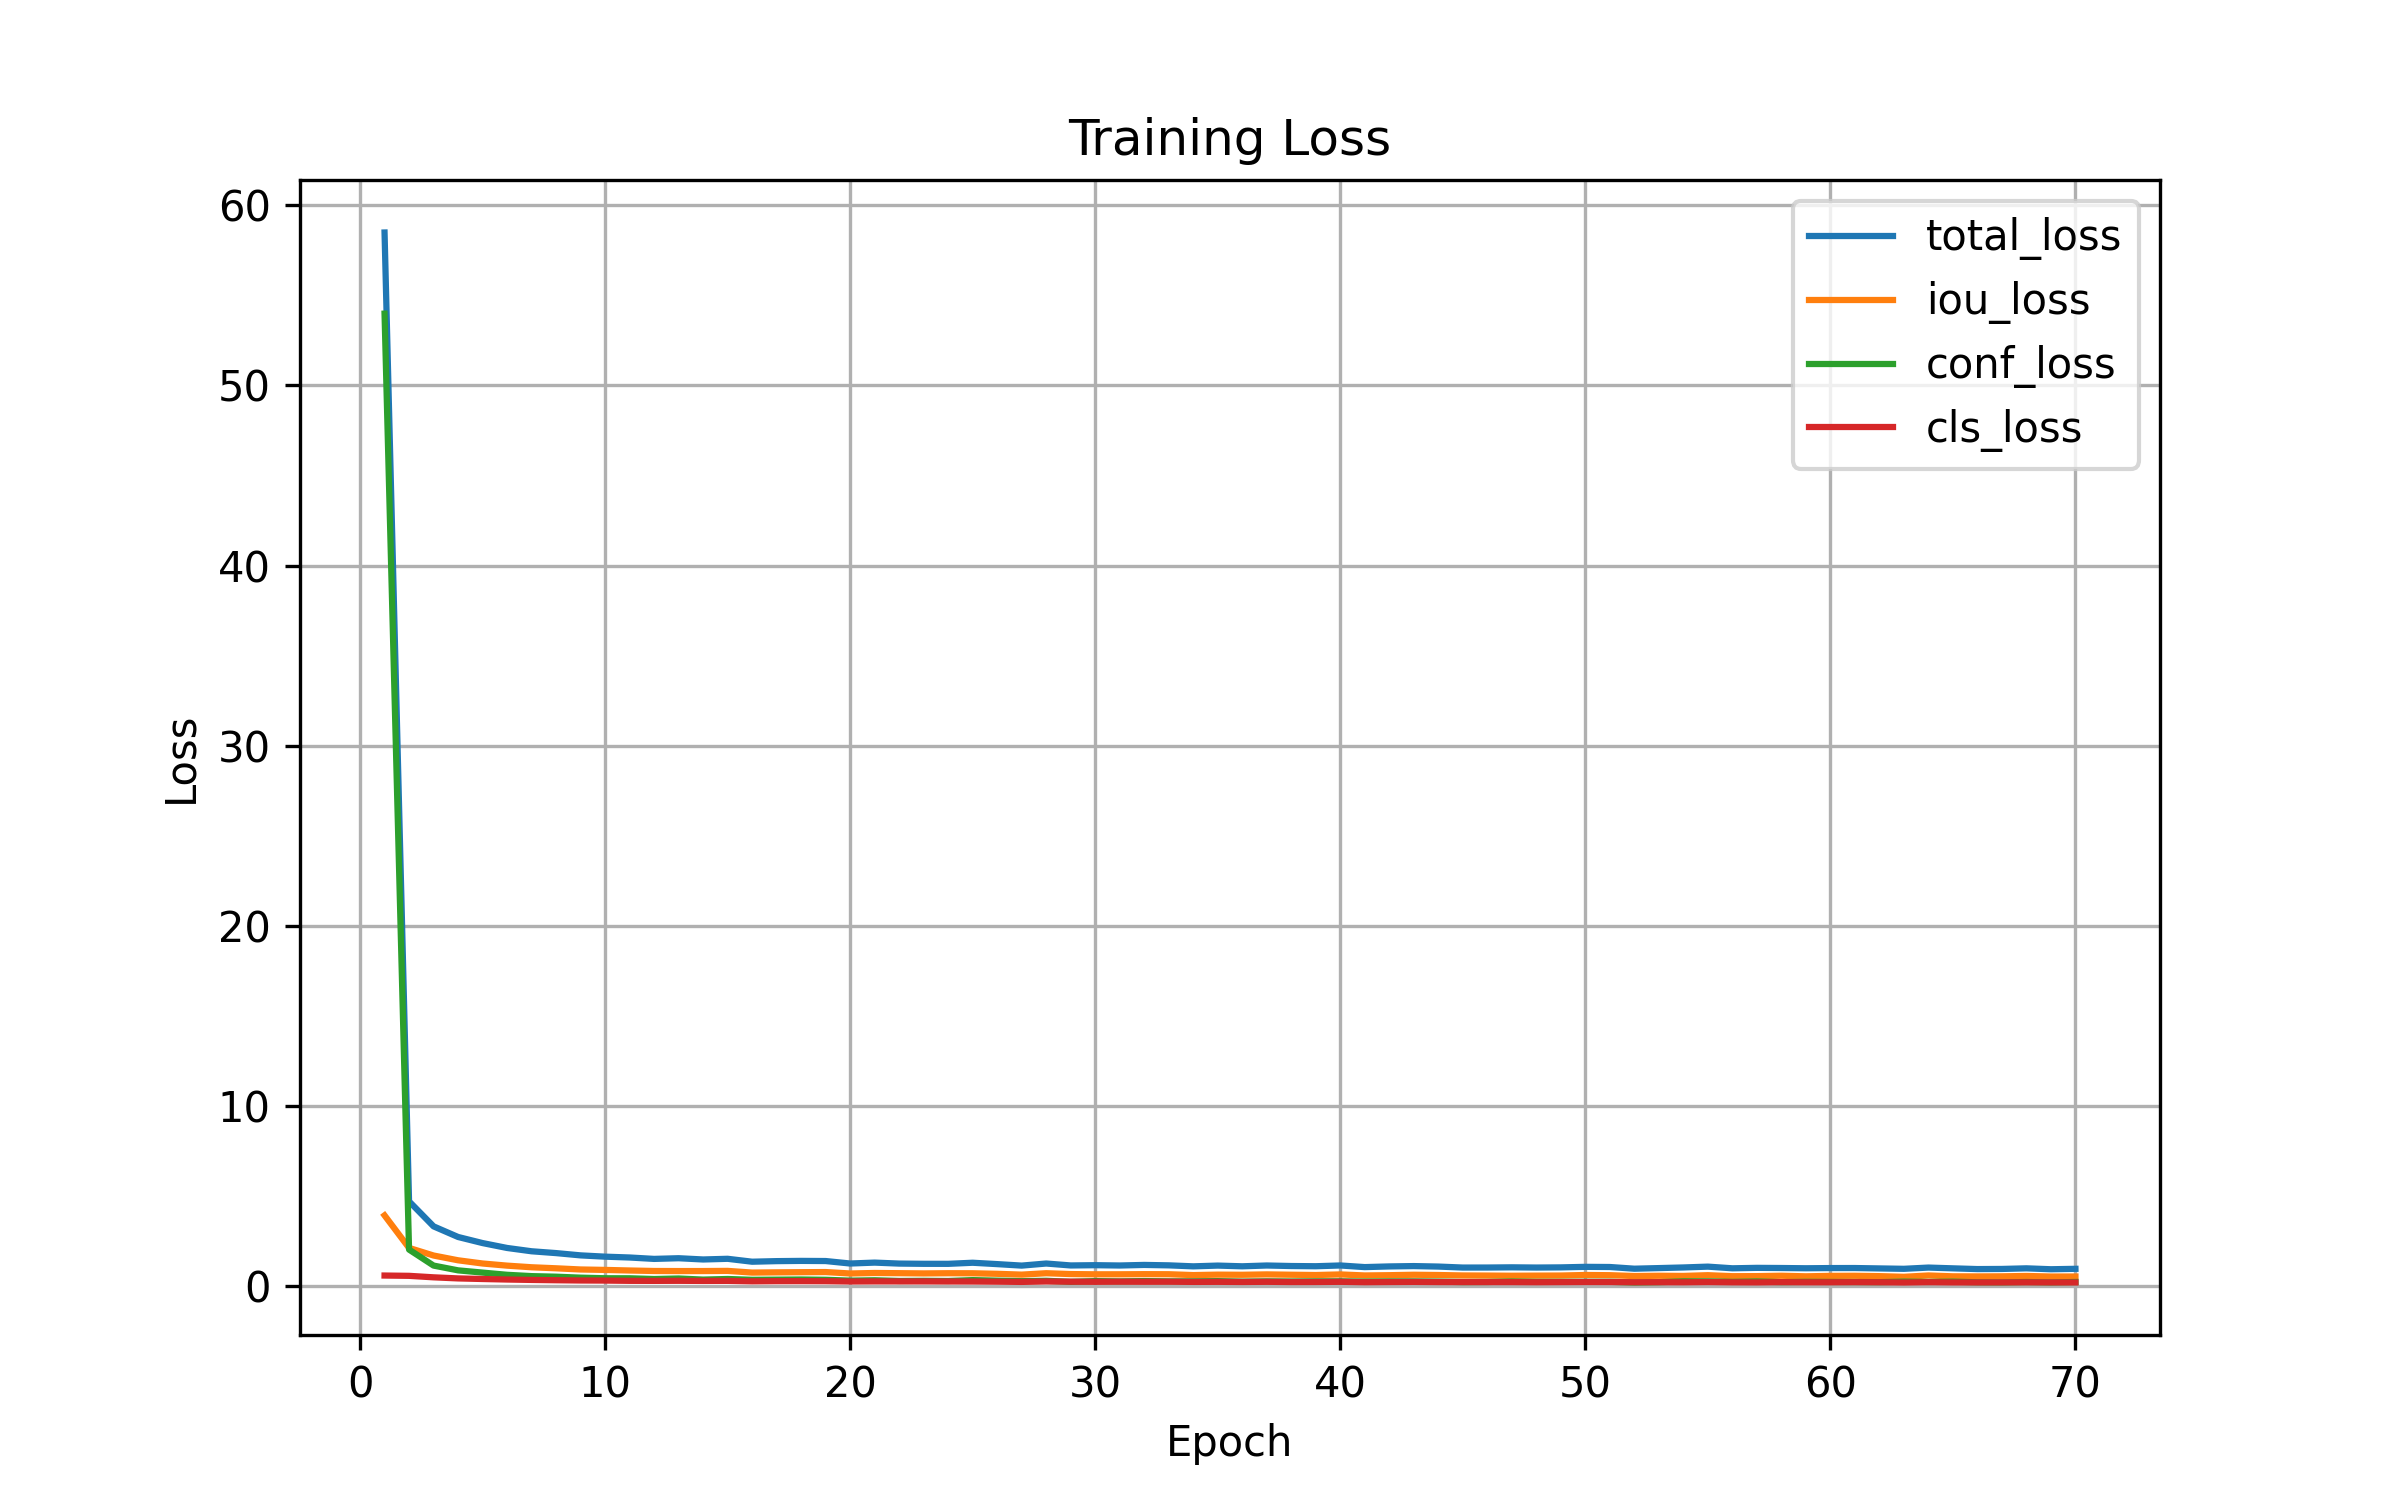
\includegraphics[width=\linewidth]{figures/images/chapter-11/qr-bar/v0/loss_curve.png}
\caption{Training loss}
\end{subfigure}
\hfill
\begin{subfigure}{0.48\textwidth}
\centering
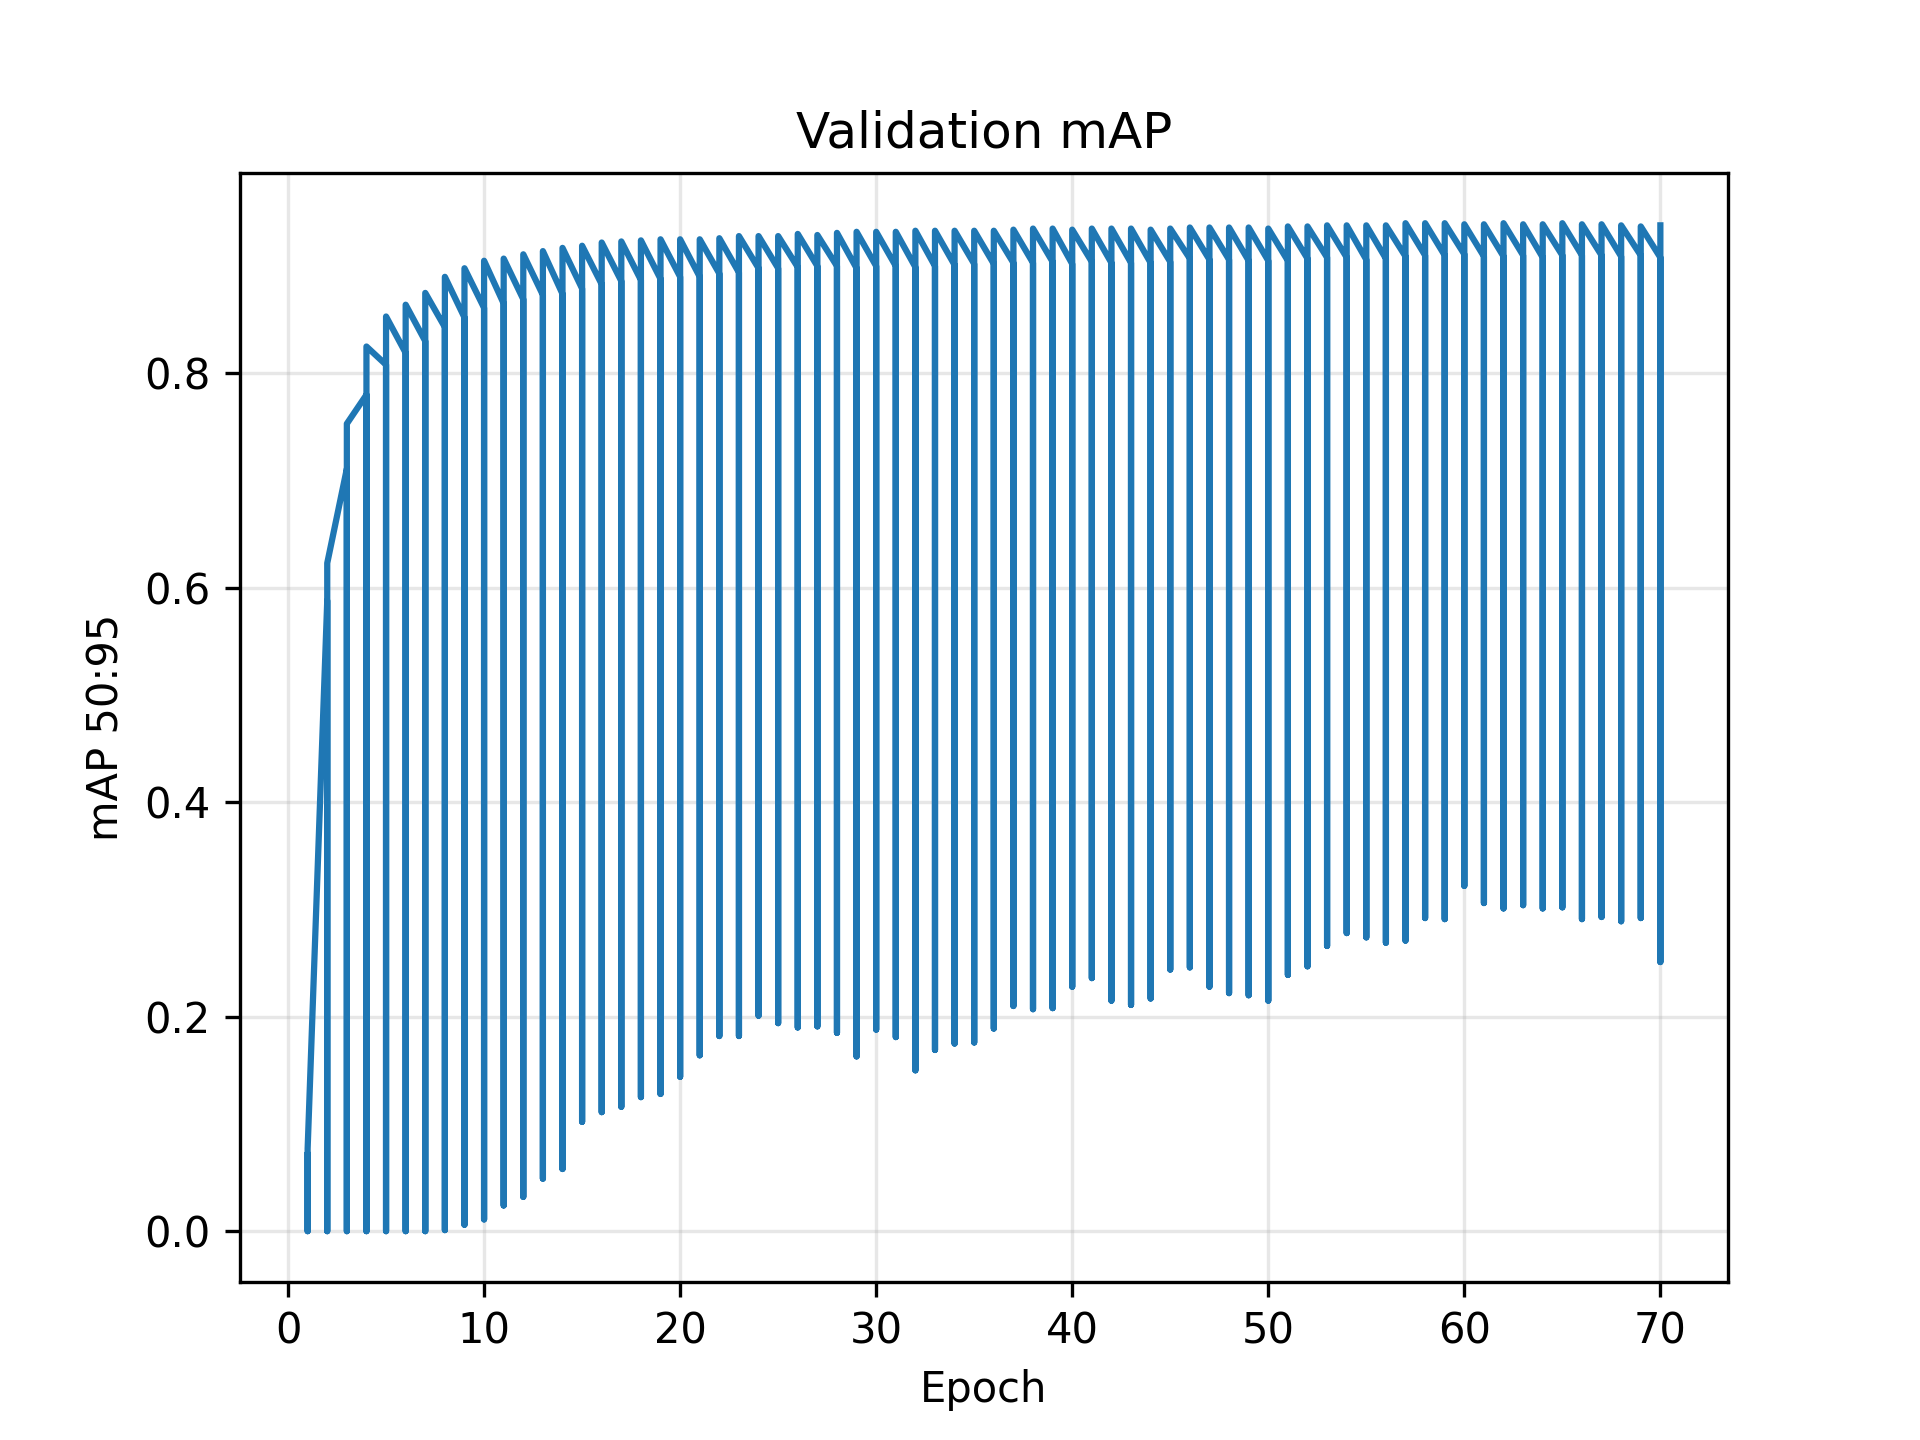
\includegraphics[width=\linewidth]{figures/images/chapter-11/qr-bar/v0/map_curve.png}
\caption{Validation mAP}
\end{subfigure}

\vspace{0.4cm}

\begin{subfigure}{0.50\textwidth}
\centering
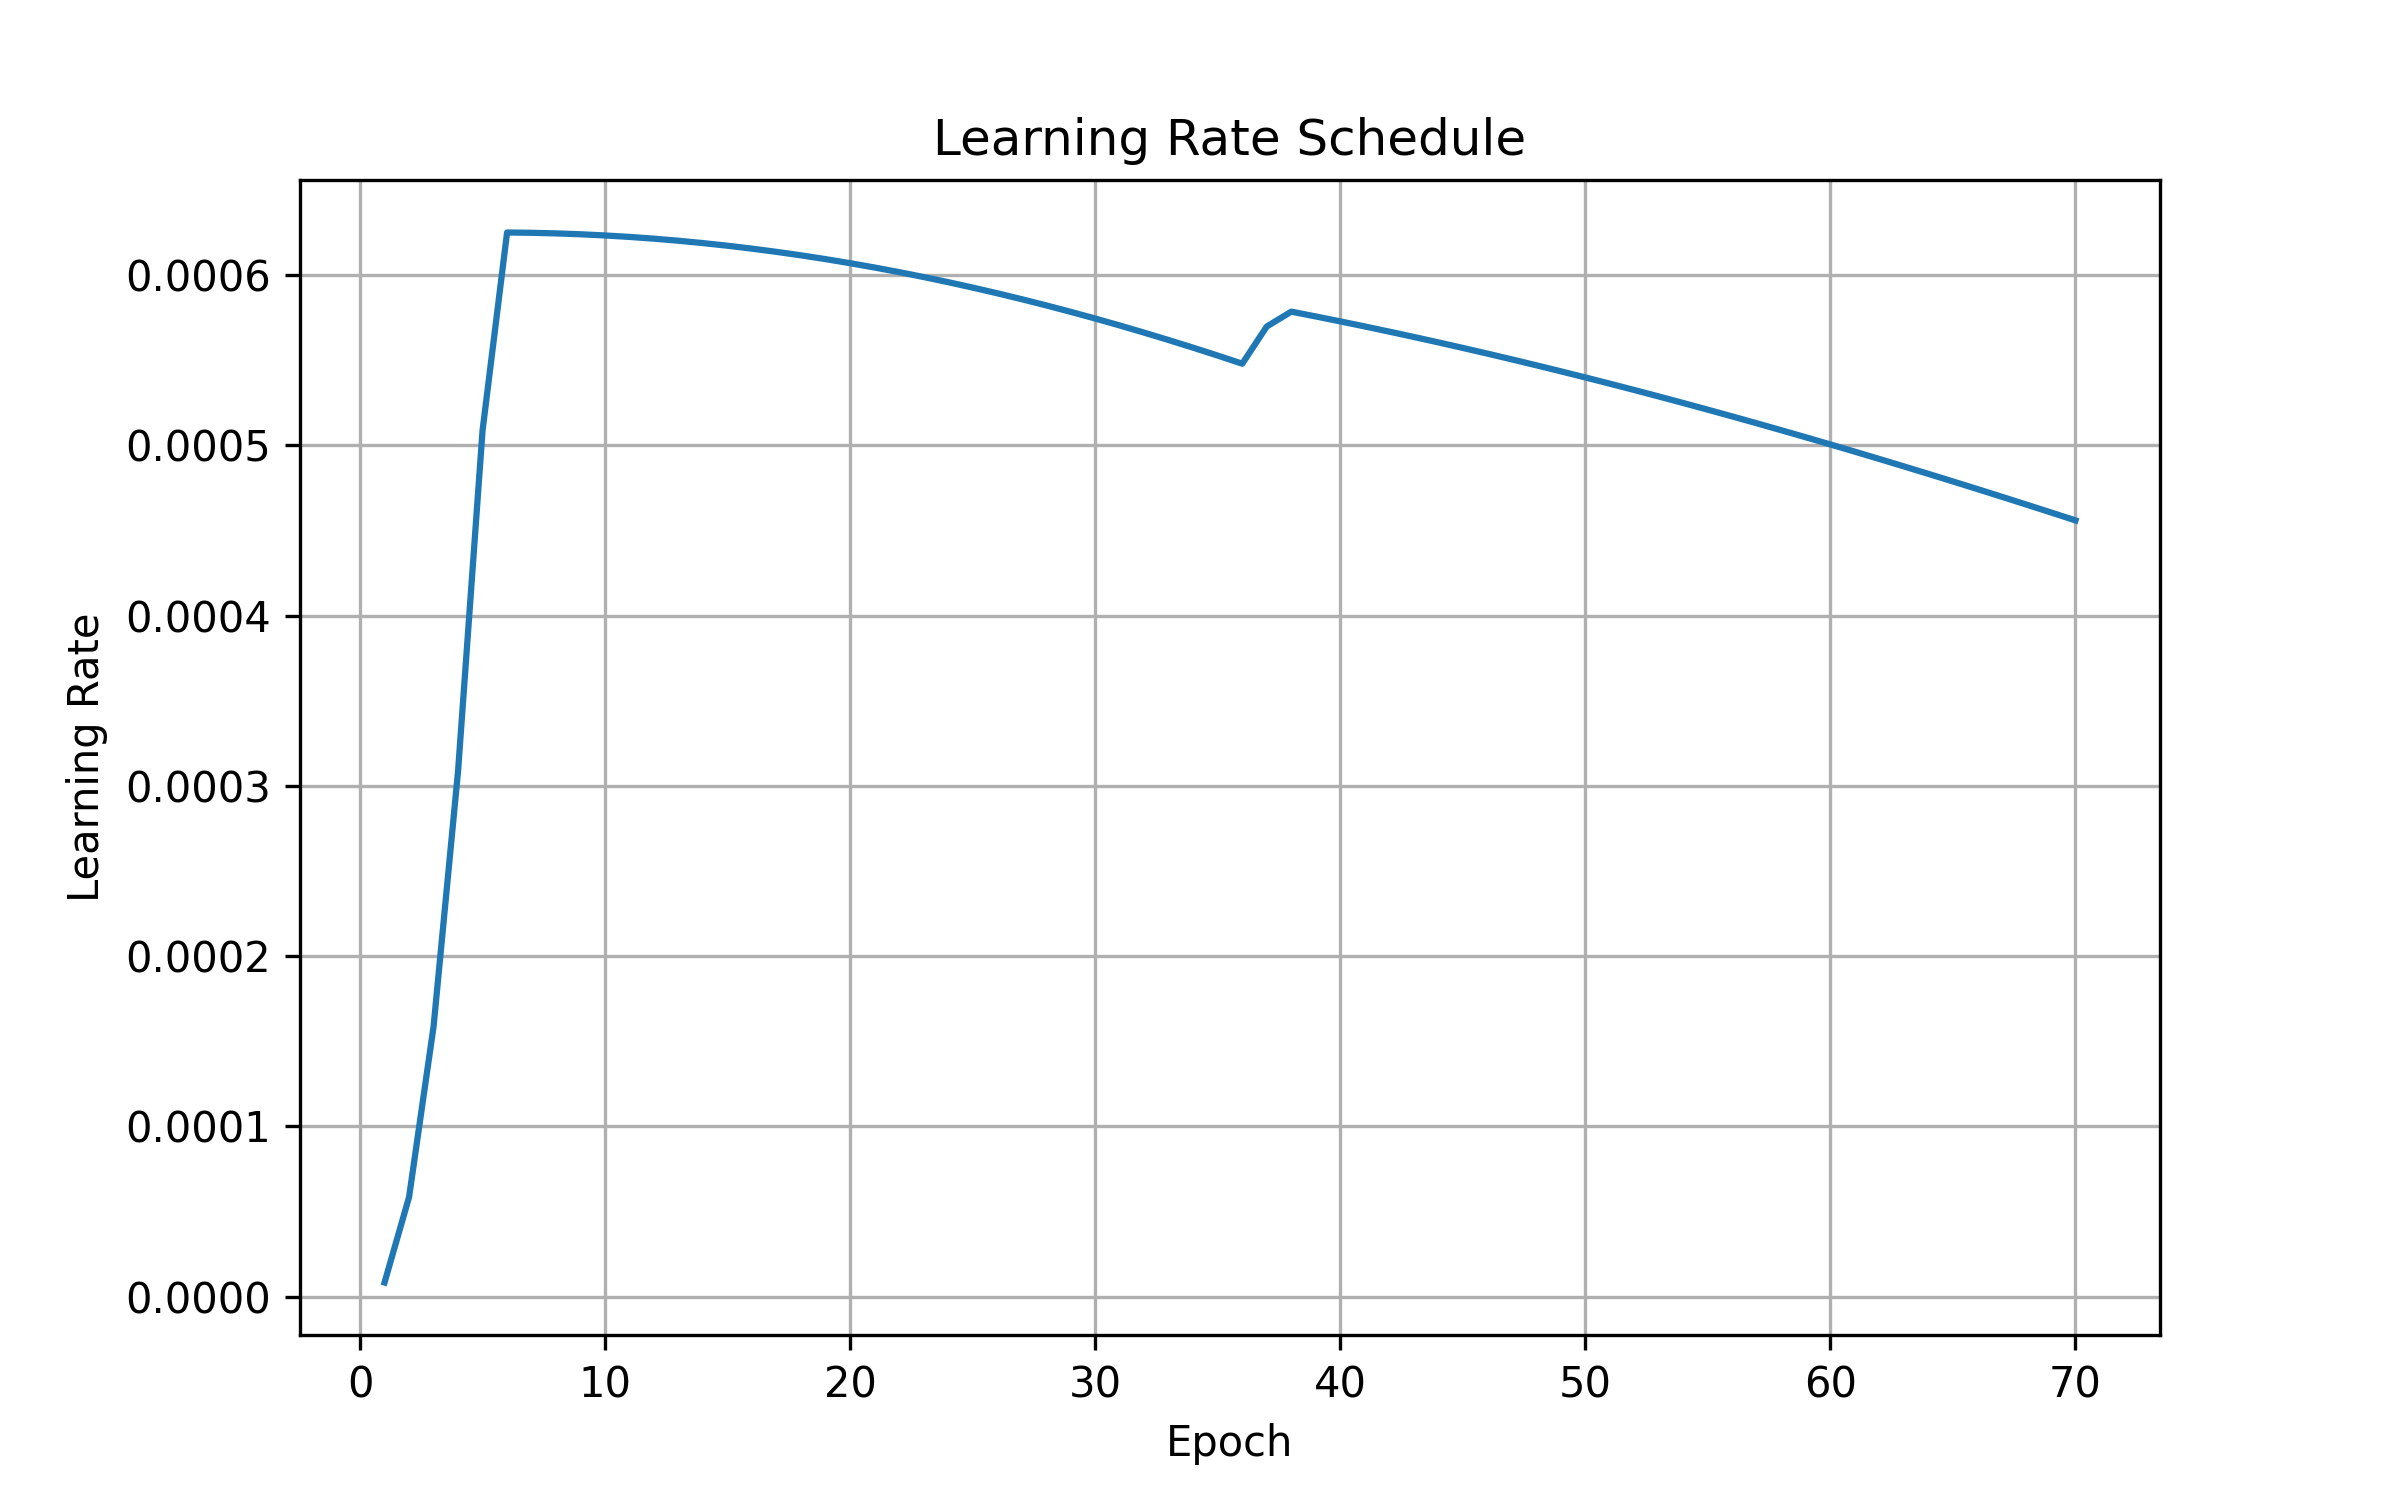
\includegraphics[width=\linewidth]{figures/images/chapter-11/qr-bar/v0/lr_curve.png}
\caption{Learning rate schedule}
\end{subfigure}

\caption{Training behaviour of the final barcode detection model.}
\label{fig:bc_training}
\end{figure}

The training loss decreases rapidly during the initial epochs and gradually
stabilizes, indicating successful convergence of the model.

The validation mAP increases quickly and stabilizes at a high level, showing
that the model generalizes well to unseen data.



\subsection{Precision--Recall Analysis}

\begin{figure}[H]
\centering
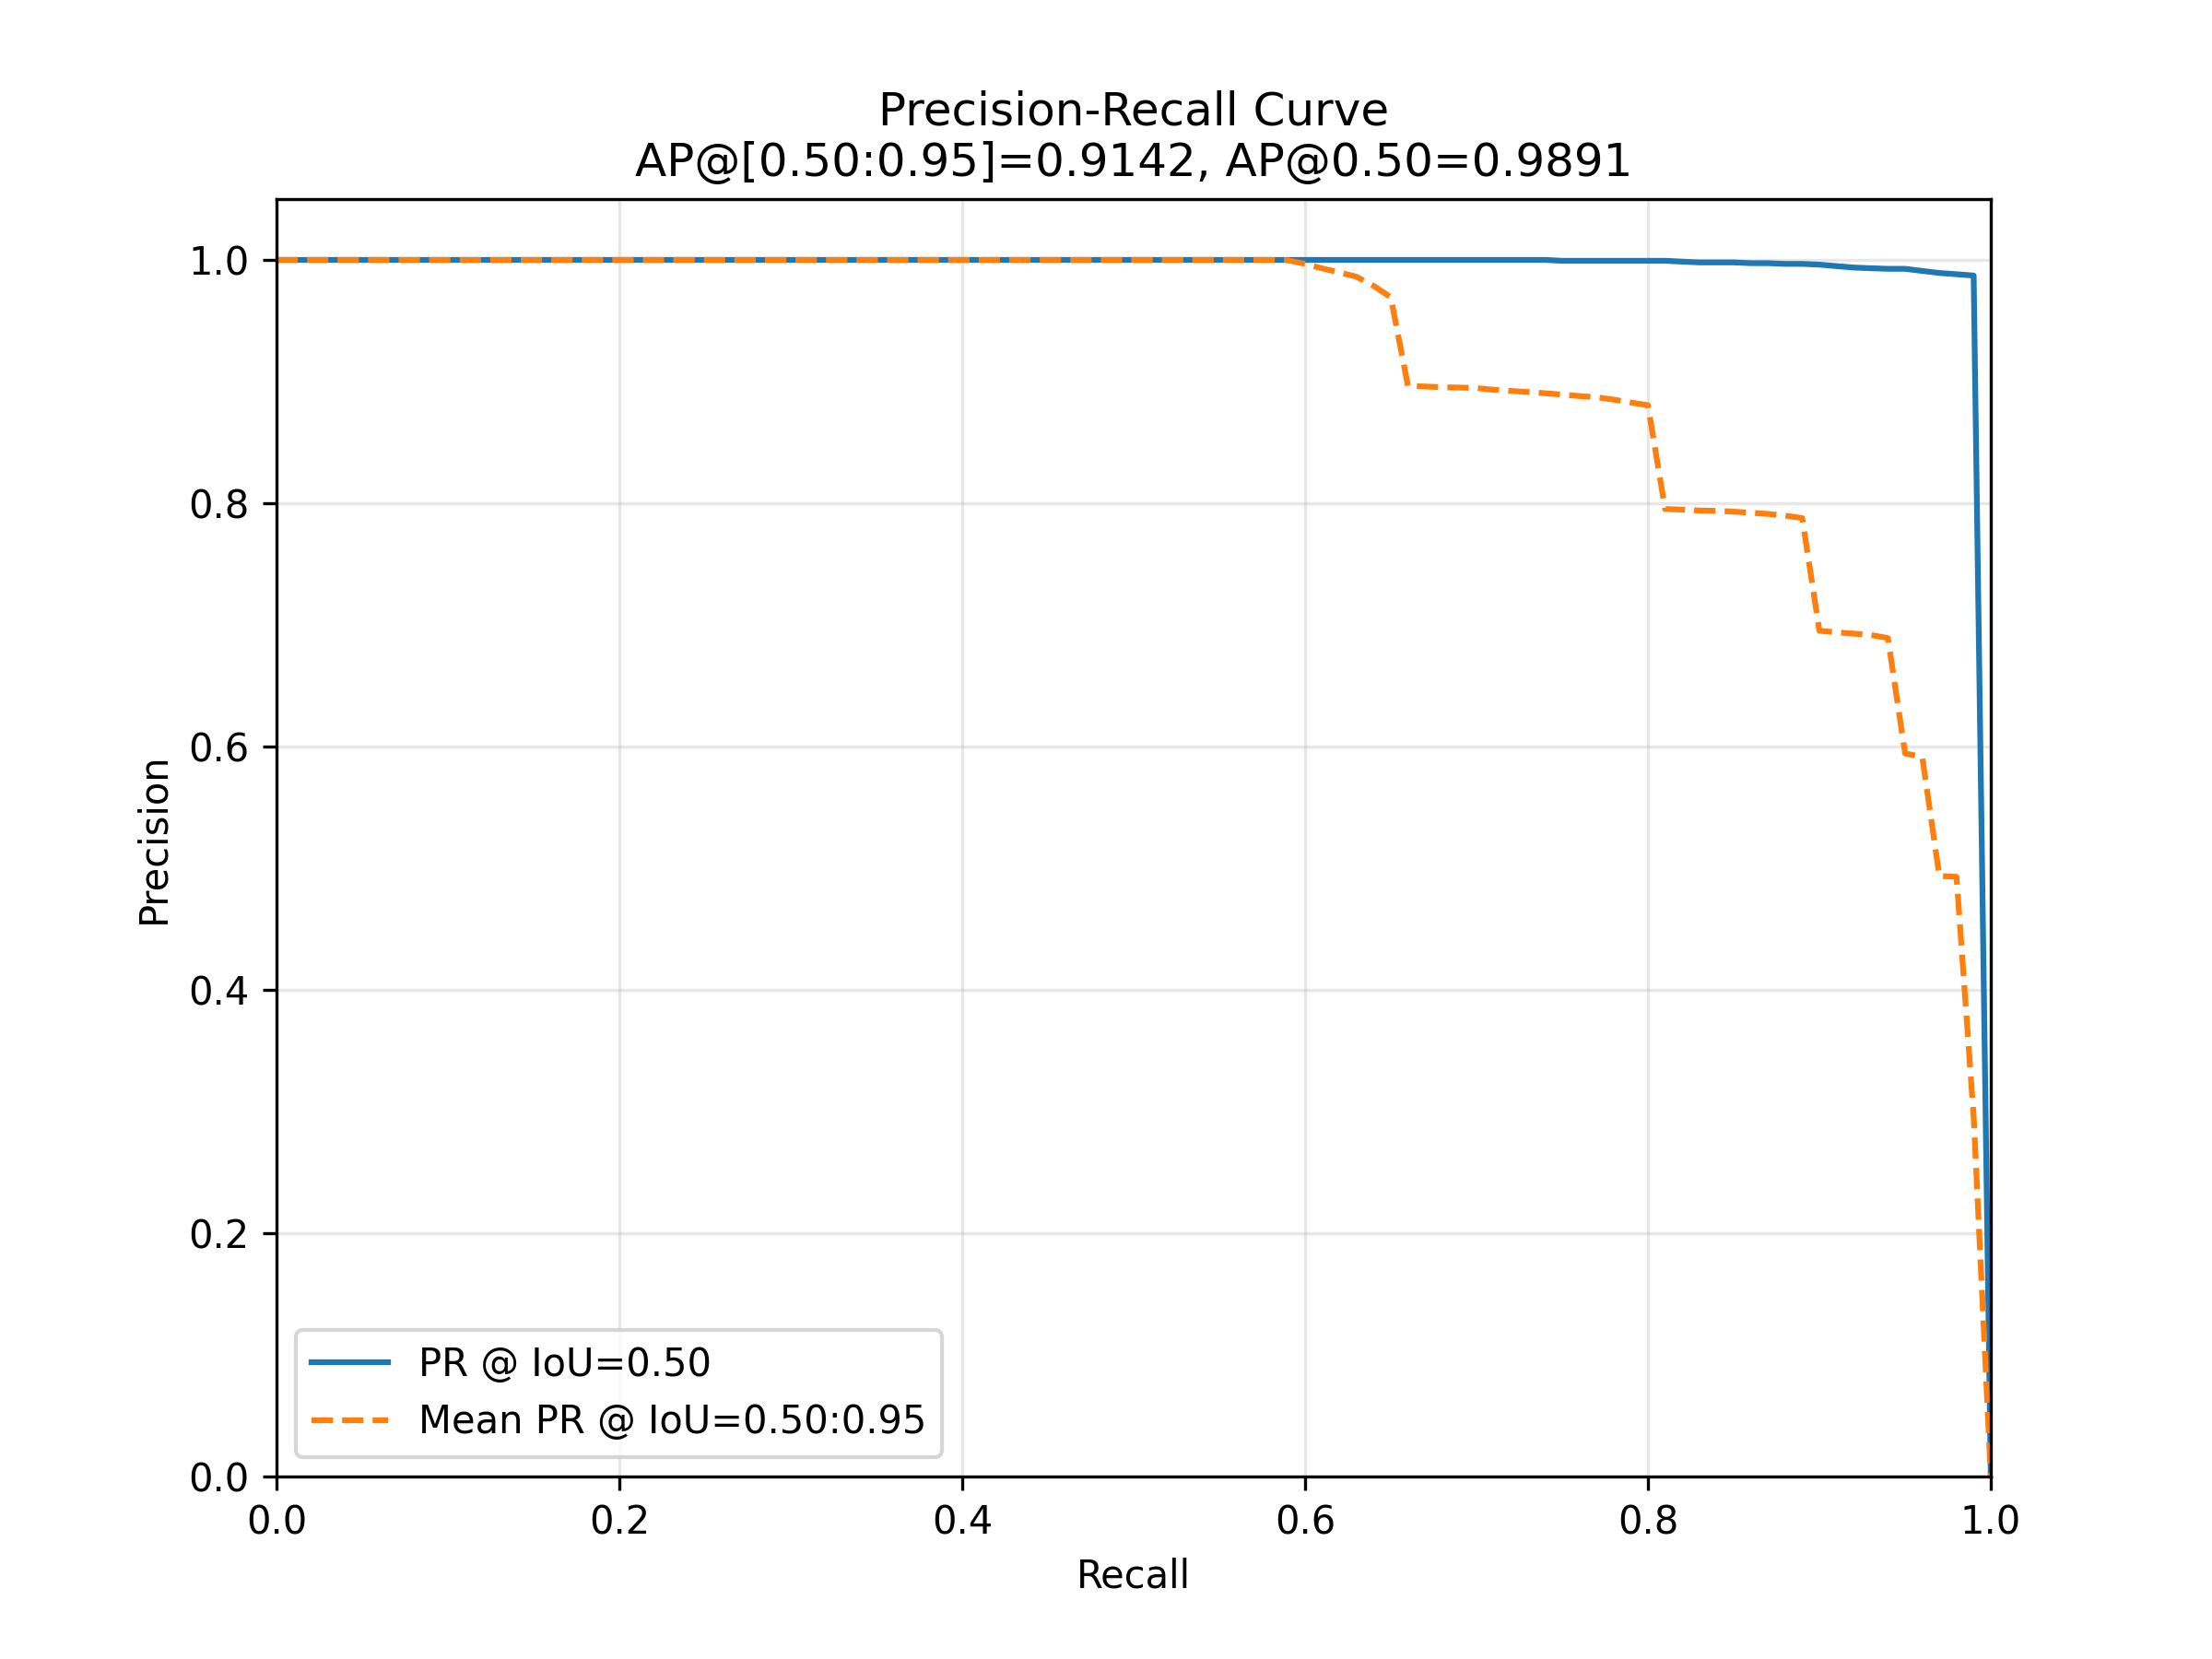
\includegraphics[width=10cm]{figures/images/chapter-11/qr-bar/v0/pr_curve.png}
\caption{Precision--recall curve for the barcode detection model.}
\label{fig:bc_pr_curve}
\end{figure}

The model achieves a high Average Precision, with
$AP@0.50 = 0.989$ and $AP@0.50:0.95 \approx 0.91$,
indicating strong detection performance across different IoU thresholds.




\subsection{Confusion Matrix Analysis}

\begin{figure}[H]
\centering
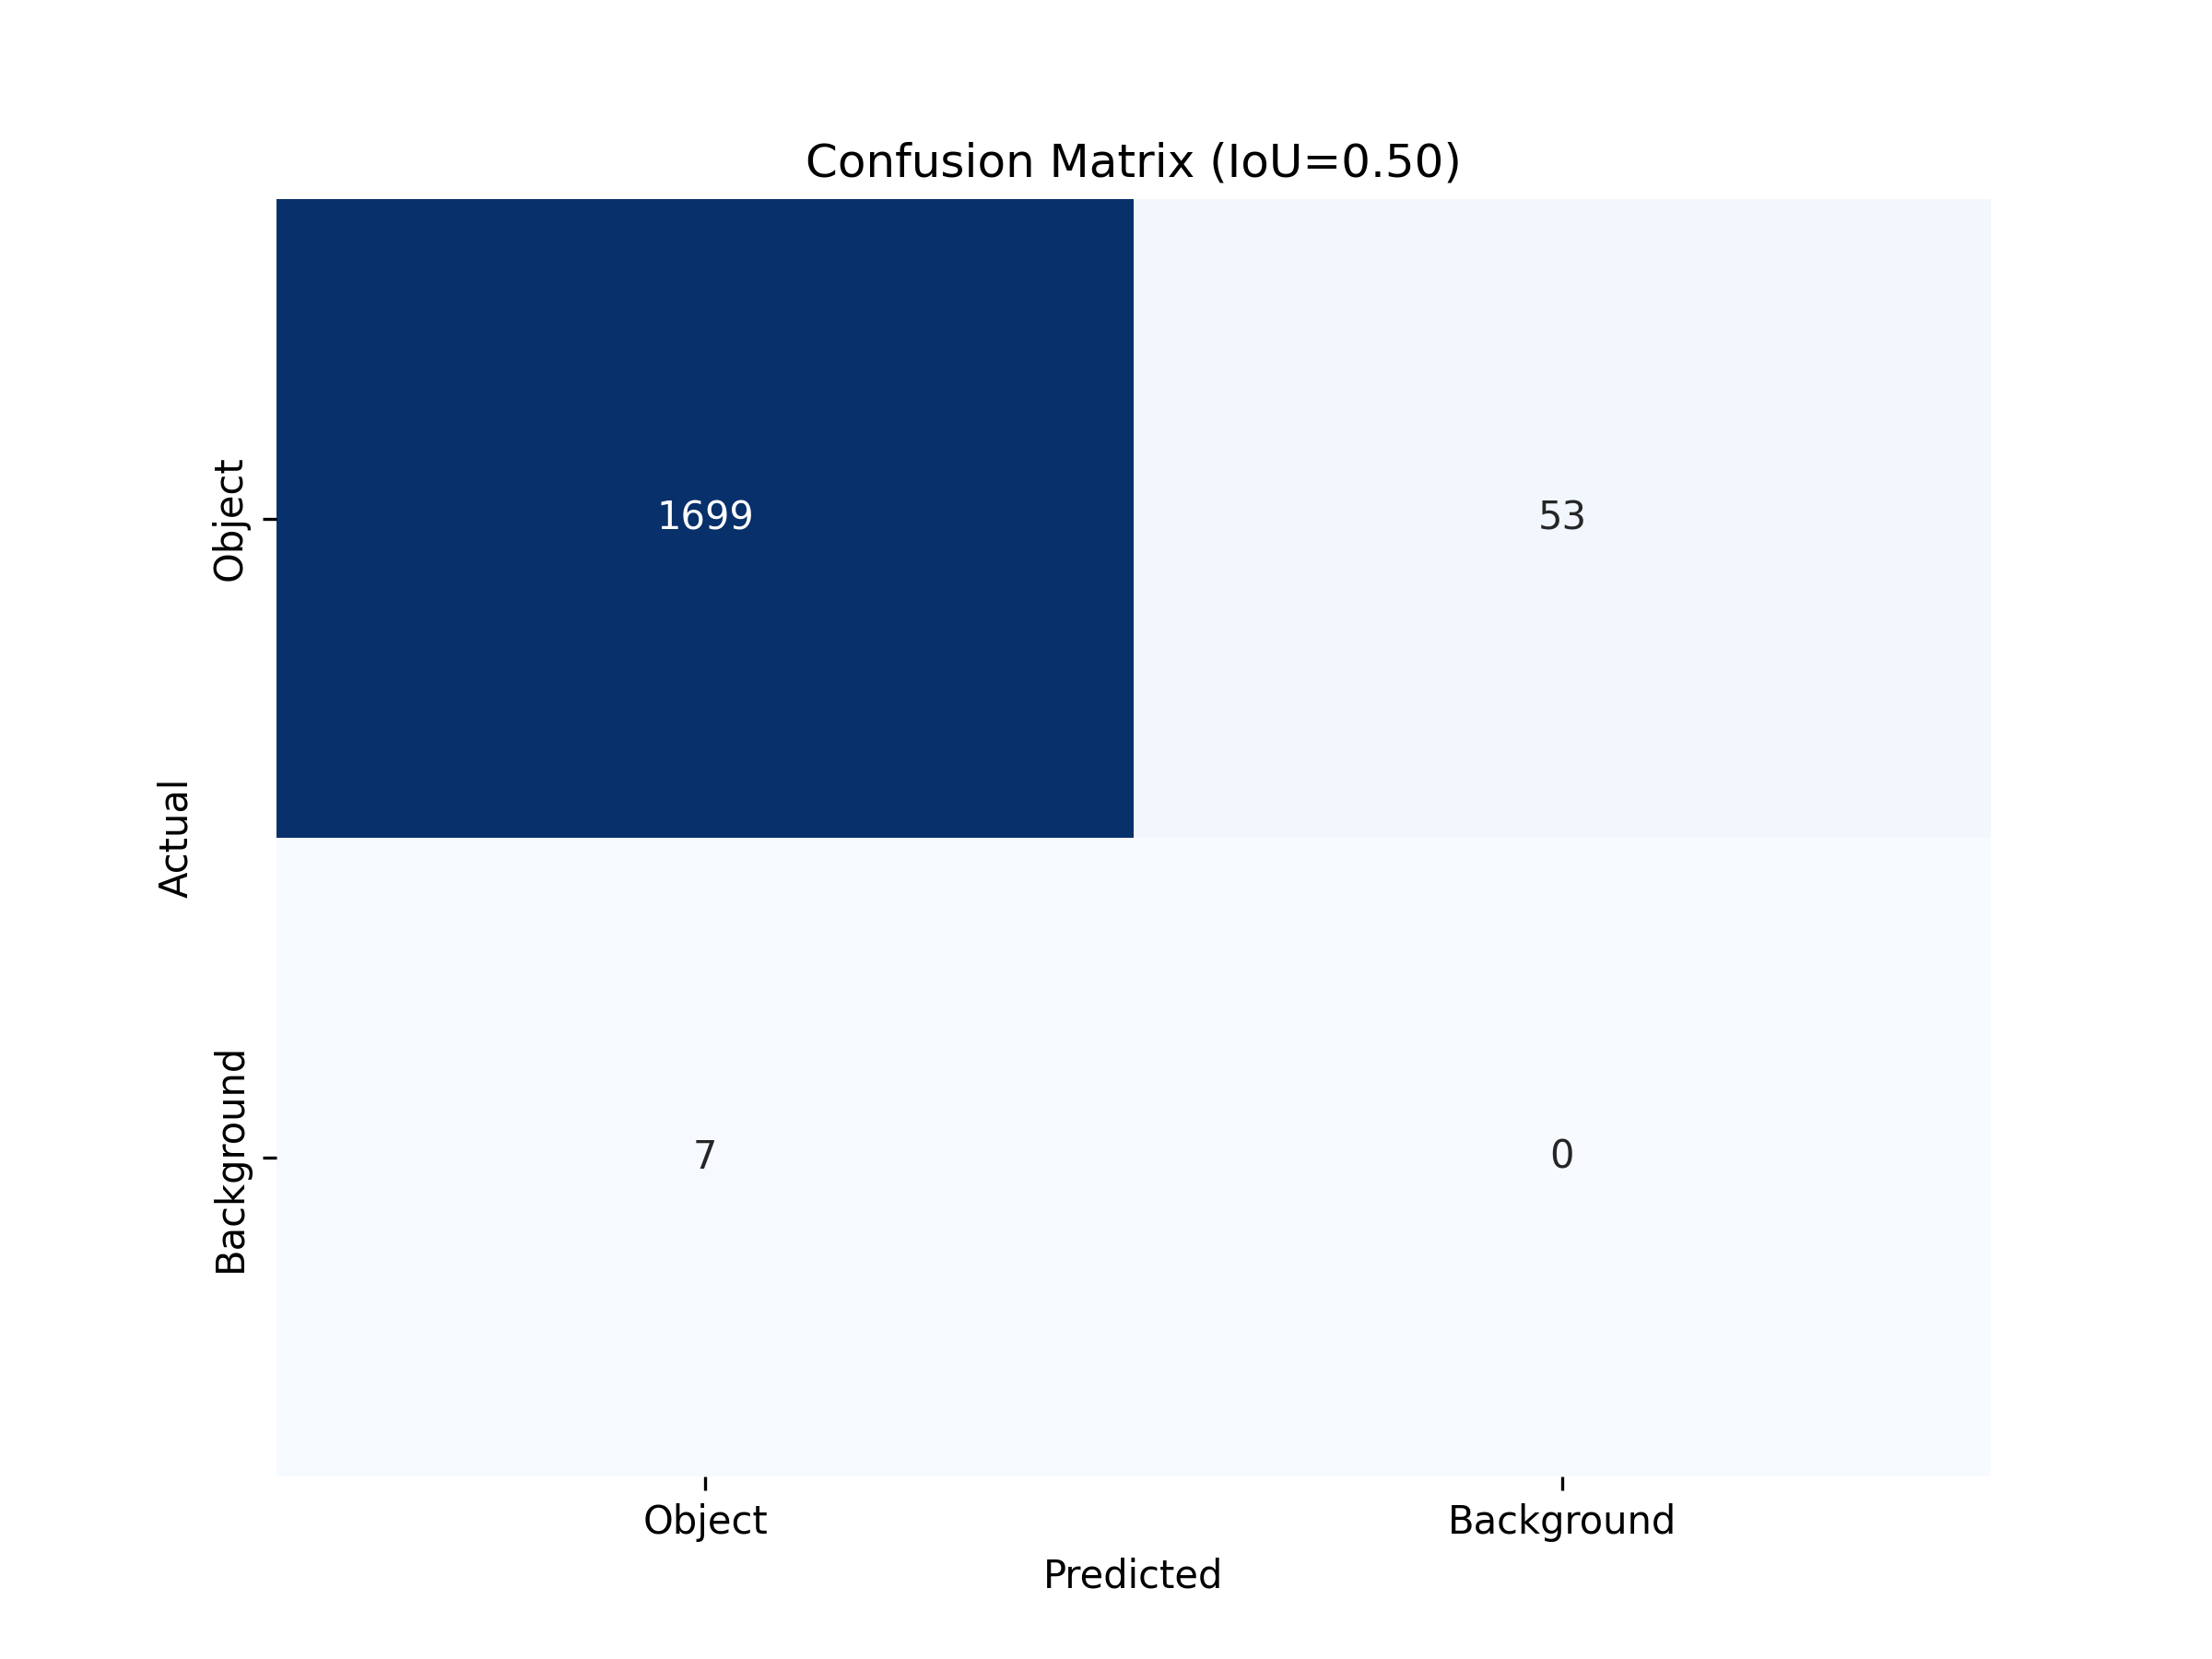
\includegraphics[width=12cm]{figures/images/chapter-11/qr-bar/v0/confusion_matrix_0.3.png}
\caption{Confusion matrix for the barcode detection model.}
\label{fig:bc_confusion_matrix}
\end{figure}

The model correctly detected 1699 barcodes, produced 53 false positives,
and missed 7 barcodes.

\begin{align*}
Precision &= \frac{1699}{1699 + 53} \approx 0.9697 \\
Recall &= \frac{1699}{1699 + 7} \approx 0.9959 \\
F1 &= 0.983
\end{align*}

\subsection{Summary}

The final barcode detection model achieved strong performance on the unseen
test set. At a confidence threshold of 0.3, the model obtained a precision of
96.97\%, a recall of 99.59\%, and an F1-score of 0.983.

The high recall indicates that the model missed very few barcodes, while the
high precision shows that most predicted detections were correct. Combined with
the high Average Precision values, these results indicate that the barcode
detector is suitable for use in the proposed system.






% ------------------------------------------------------------------------


\section{License Plate Detection}
\label{app:license_plate_results}

This section documents the detailed training and evaluation results for the
custom-trained license plate detection models. The model was trained using the
same YOLOX-based training pipeline as the barcode detection model. Therefore,
this section focuses on the supporting results used to evaluate and compare the
license plate detector configurations.


\subsection{Training Setup}

\begin{table}[H]
\centering
\begin{tabular}{l l p{5.0cm}}
\toprule
\textbf{Dataset} & \textbf{Source} & \textbf{Description} \\
\midrule
License Plate Detection Dataset
& Kaggle \cite{lp_dataset_1} 
& Dataset containing annotated license plate images from real-world environments, designed for object detection tasks \\

Large License Plate Detection Dataset
& Kaggle \cite{lp_dataset_2} 
& Large-scale dataset with diverse license plate instances captured under varying lighting and environmental conditions \\

\midrule
\textbf{Total} & 38025 & Combined into a unified dataset for training and evaluation \\
\bottomrule
\end{tabular}
\caption{Overview of datasets used for training the license plate detection model.}
\label{tab:licenseplate_datasets}
\end{table}



The dataset was divided into approximately 85\% training, 10\% validation, and
5\% testing. After excluding three label files, the dataset consisted of 36,959 images. This split was chosen to provide a large number of training
samples while still reserving separate validation and test sets for monitoring
training performance and evaluating the final model on unseen data. Both models
used the same training, validation, and test split.


\begin{table}[H]
\centering

\begin{minipage}[t]{0.43\textwidth}
\centering
\caption{Training Configuration for Model V0}
\label{tab:lp_training_config_v0}
\scriptsize
\renewcommand{\arraystretch}{1.05}
\begin{tabular}{>{\raggedright\arraybackslash}p{0.52\linewidth}
                >{\raggedright\arraybackslash}p{0.38\linewidth}}
\toprule
\textbf{Parameter} & \textbf{Value} \\
\midrule
Architecture & YOLOX-S \\
Input Resolution & $640 \times 640$ \\
Batch Size & 16 \\
Max Epochs & 200 \\
No-Aug. Epochs & 15 \\
\midrule
\textit{Optimization} & \\
Base Learning Rate & 0.01 / 64 \\
Warmup Epochs & 5 \\
Min LR Ratio & 0.05 \\
Optimizer & SGD \\
\midrule
\textit{Augmentation (Offline)} & \\
Mosaic Images & 0.8 (0.3--1.8) \\
Color / Flip & 0.5 / 0.5 \\
Rotation / Shift / Shear & 5.0 / 0.05 / 1.0 \\
Random Image Size & (10, 20) \\
\midrule
\textit{Hardware} & \\
GPU Model & RTX 4080 \\
\bottomrule
\end{tabular}
\end{minipage}
\hfill
\begin{minipage}[t]{0.43\textwidth}
\centering
\caption{Training Configuration for Model V1}
\label{tab:lp_training_config_v1}
\scriptsize
\renewcommand{\arraystretch}{1.05}
\begin{tabular}{>{\raggedright\arraybackslash}p{0.52\linewidth}
                >{\raggedright\arraybackslash}p{0.38\linewidth}}
\toprule
\textbf{Parameter} & \textbf{Value} \\
\midrule
Architecture & YOLOX-S \\
Input Resolution & $960 \times 960$ \\
Batch Size & 8 \\
Max Epochs & 200 \\
No-Aug. Epochs & 15 \\
\midrule
\textit{Optimization} & \\
Base Learning Rate & 0.01 / 64 \\
Warmup Epochs & 5 \\
Min LR Ratio & 0.05 \\
Optimizer & SGD \\
\midrule
\textit{Augmentation (Offline)} & \\
Mosaic Images & 0.8 (0.5--1.5) \\
Color / Flip & 0.5 / 0.5 \\
Rotation / Shift / Shear & 5.0 / 0.05 / 1.0 \\
Random Image Size & (14, 24) \\
\midrule
\textit{Hardware} & \\
GPU Model & RTX 4080 \\
\bottomrule
\end{tabular}
\end{minipage}

\end{table}

Tables~\ref{tab:lp_training_config_v0} and~\ref{tab:lp_training_config_v1}
summarize the training configurations for the two license plate detection
models. The main difference was the increased input resolution in v1, which
required a smaller batch size.



\subsection{Training Curves}


\begin{figure}[H]
\centering

\begin{subfigure}{0.50\textwidth}
\centering
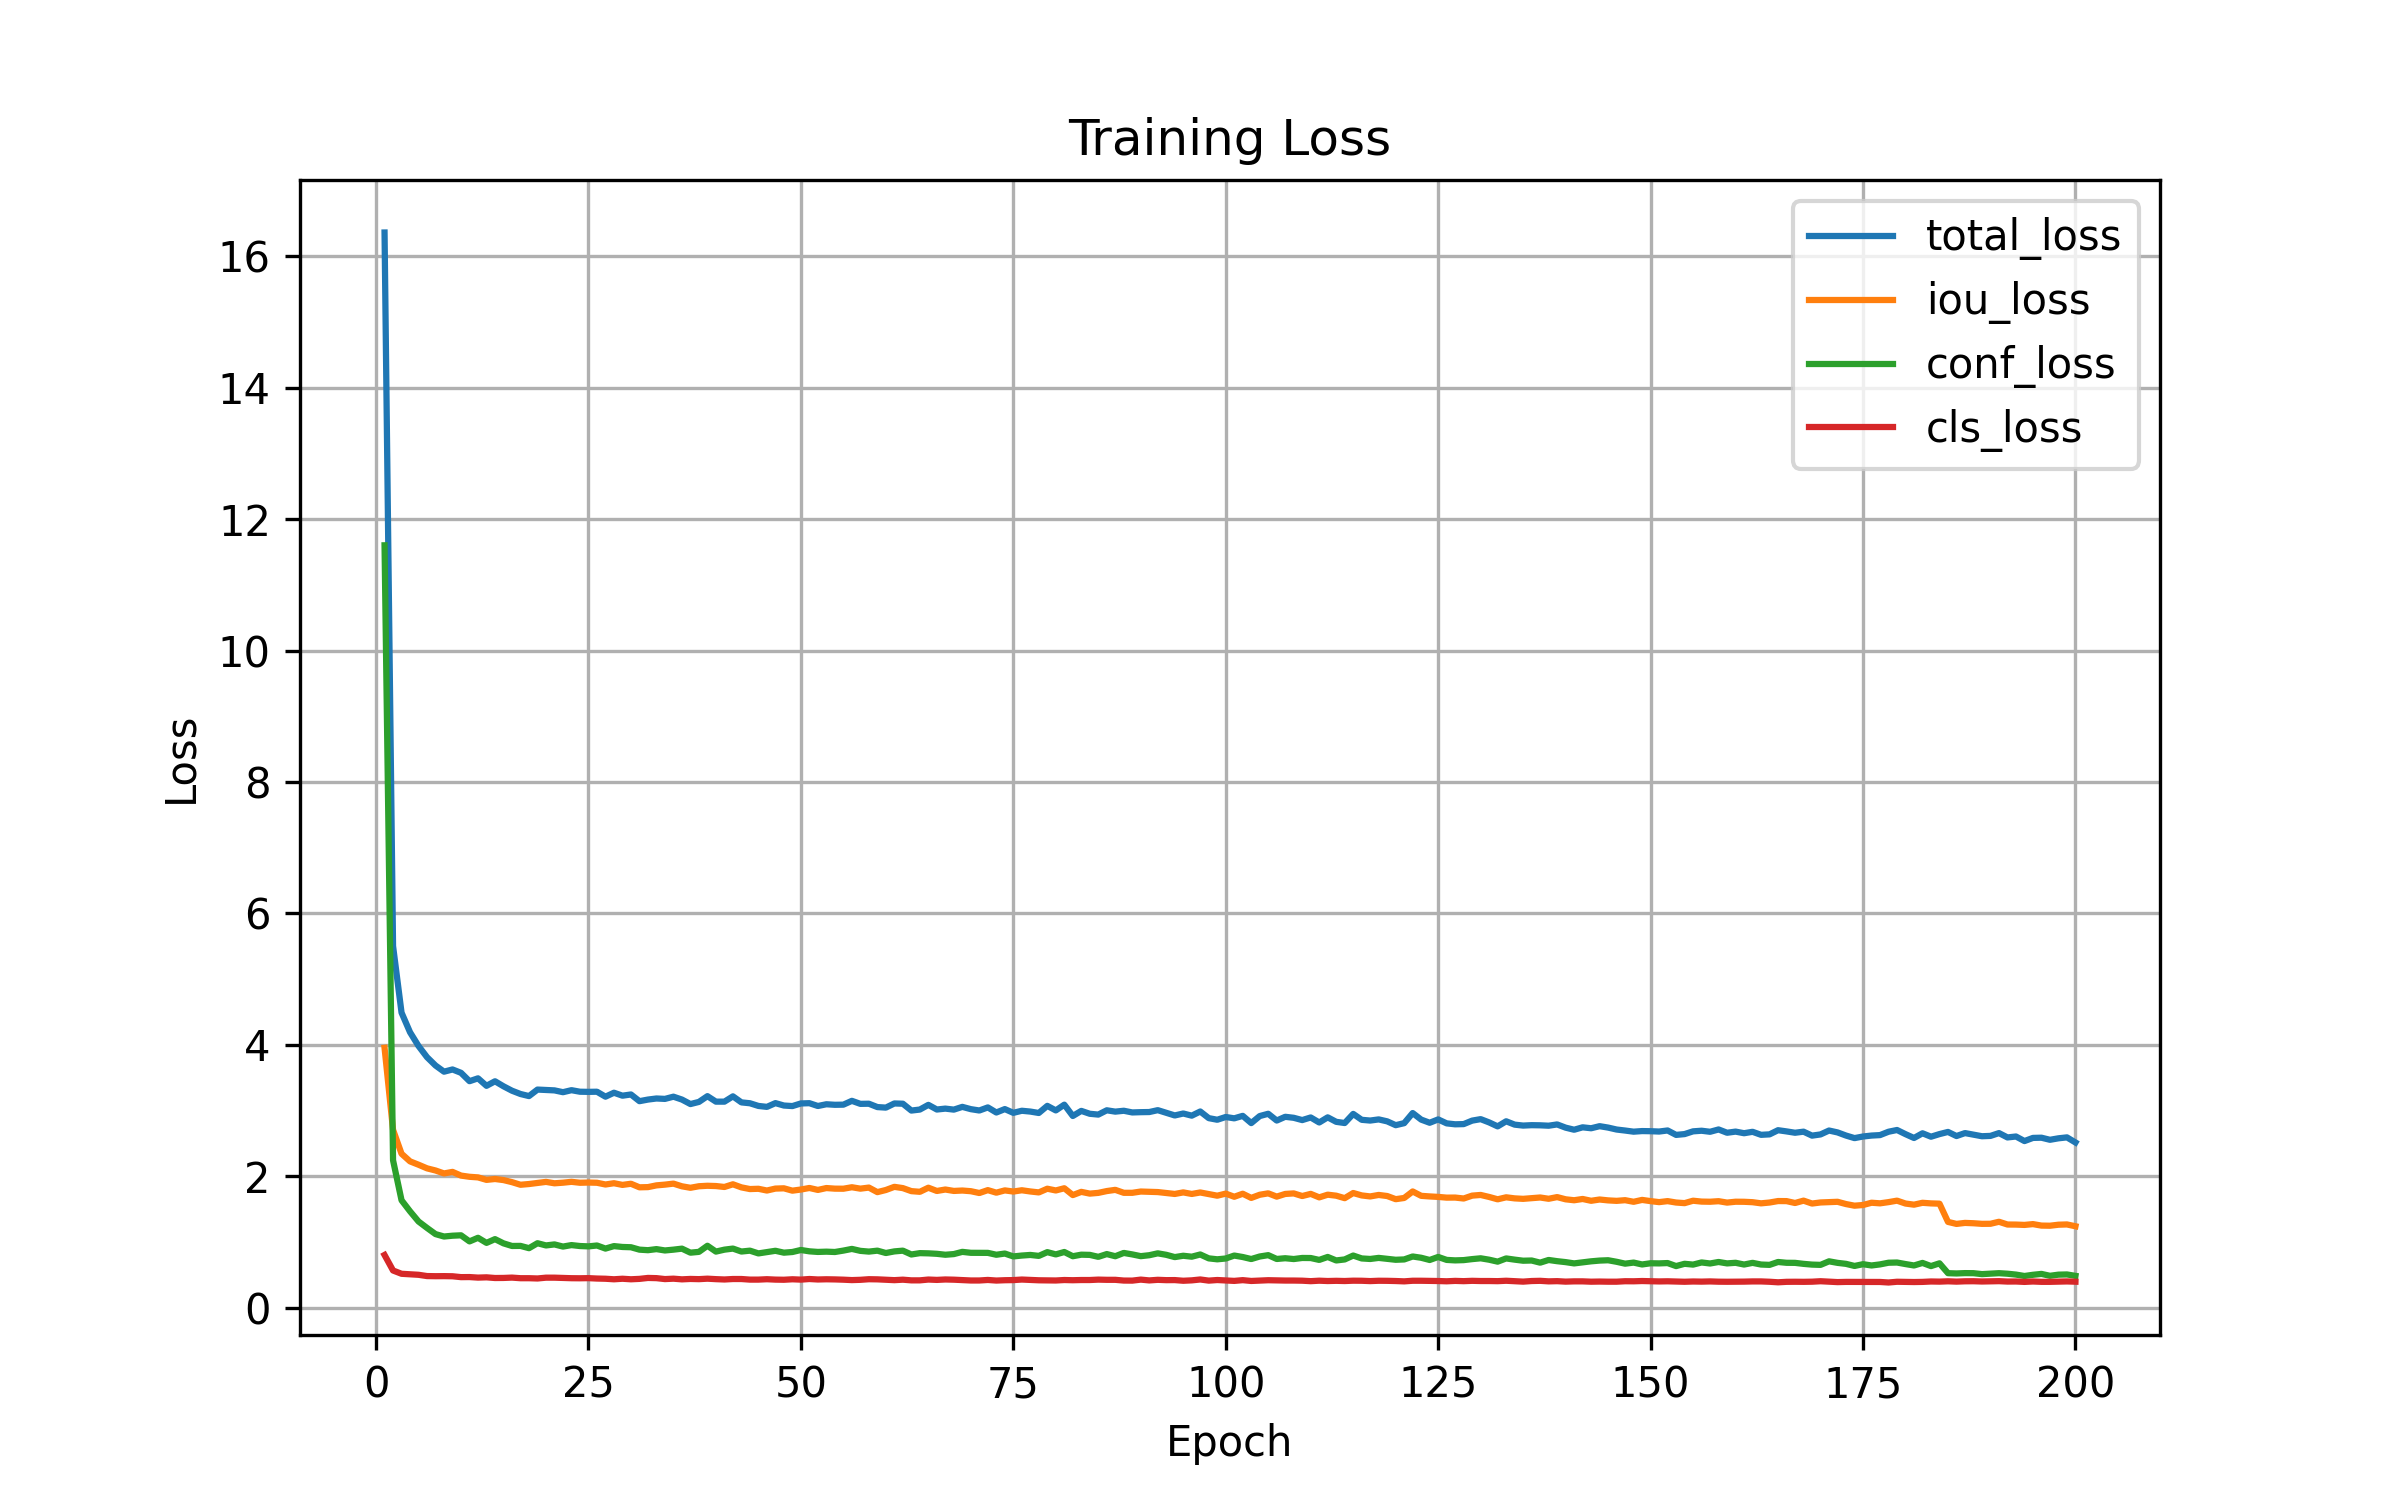
\includegraphics[width=\linewidth]{figures/images/chapter-11/licenseplate/v0/loss_curve.png}
\caption{Training loss}
\end{subfigure}
\hfill
\begin{subfigure}{0.48\textwidth}
\centering
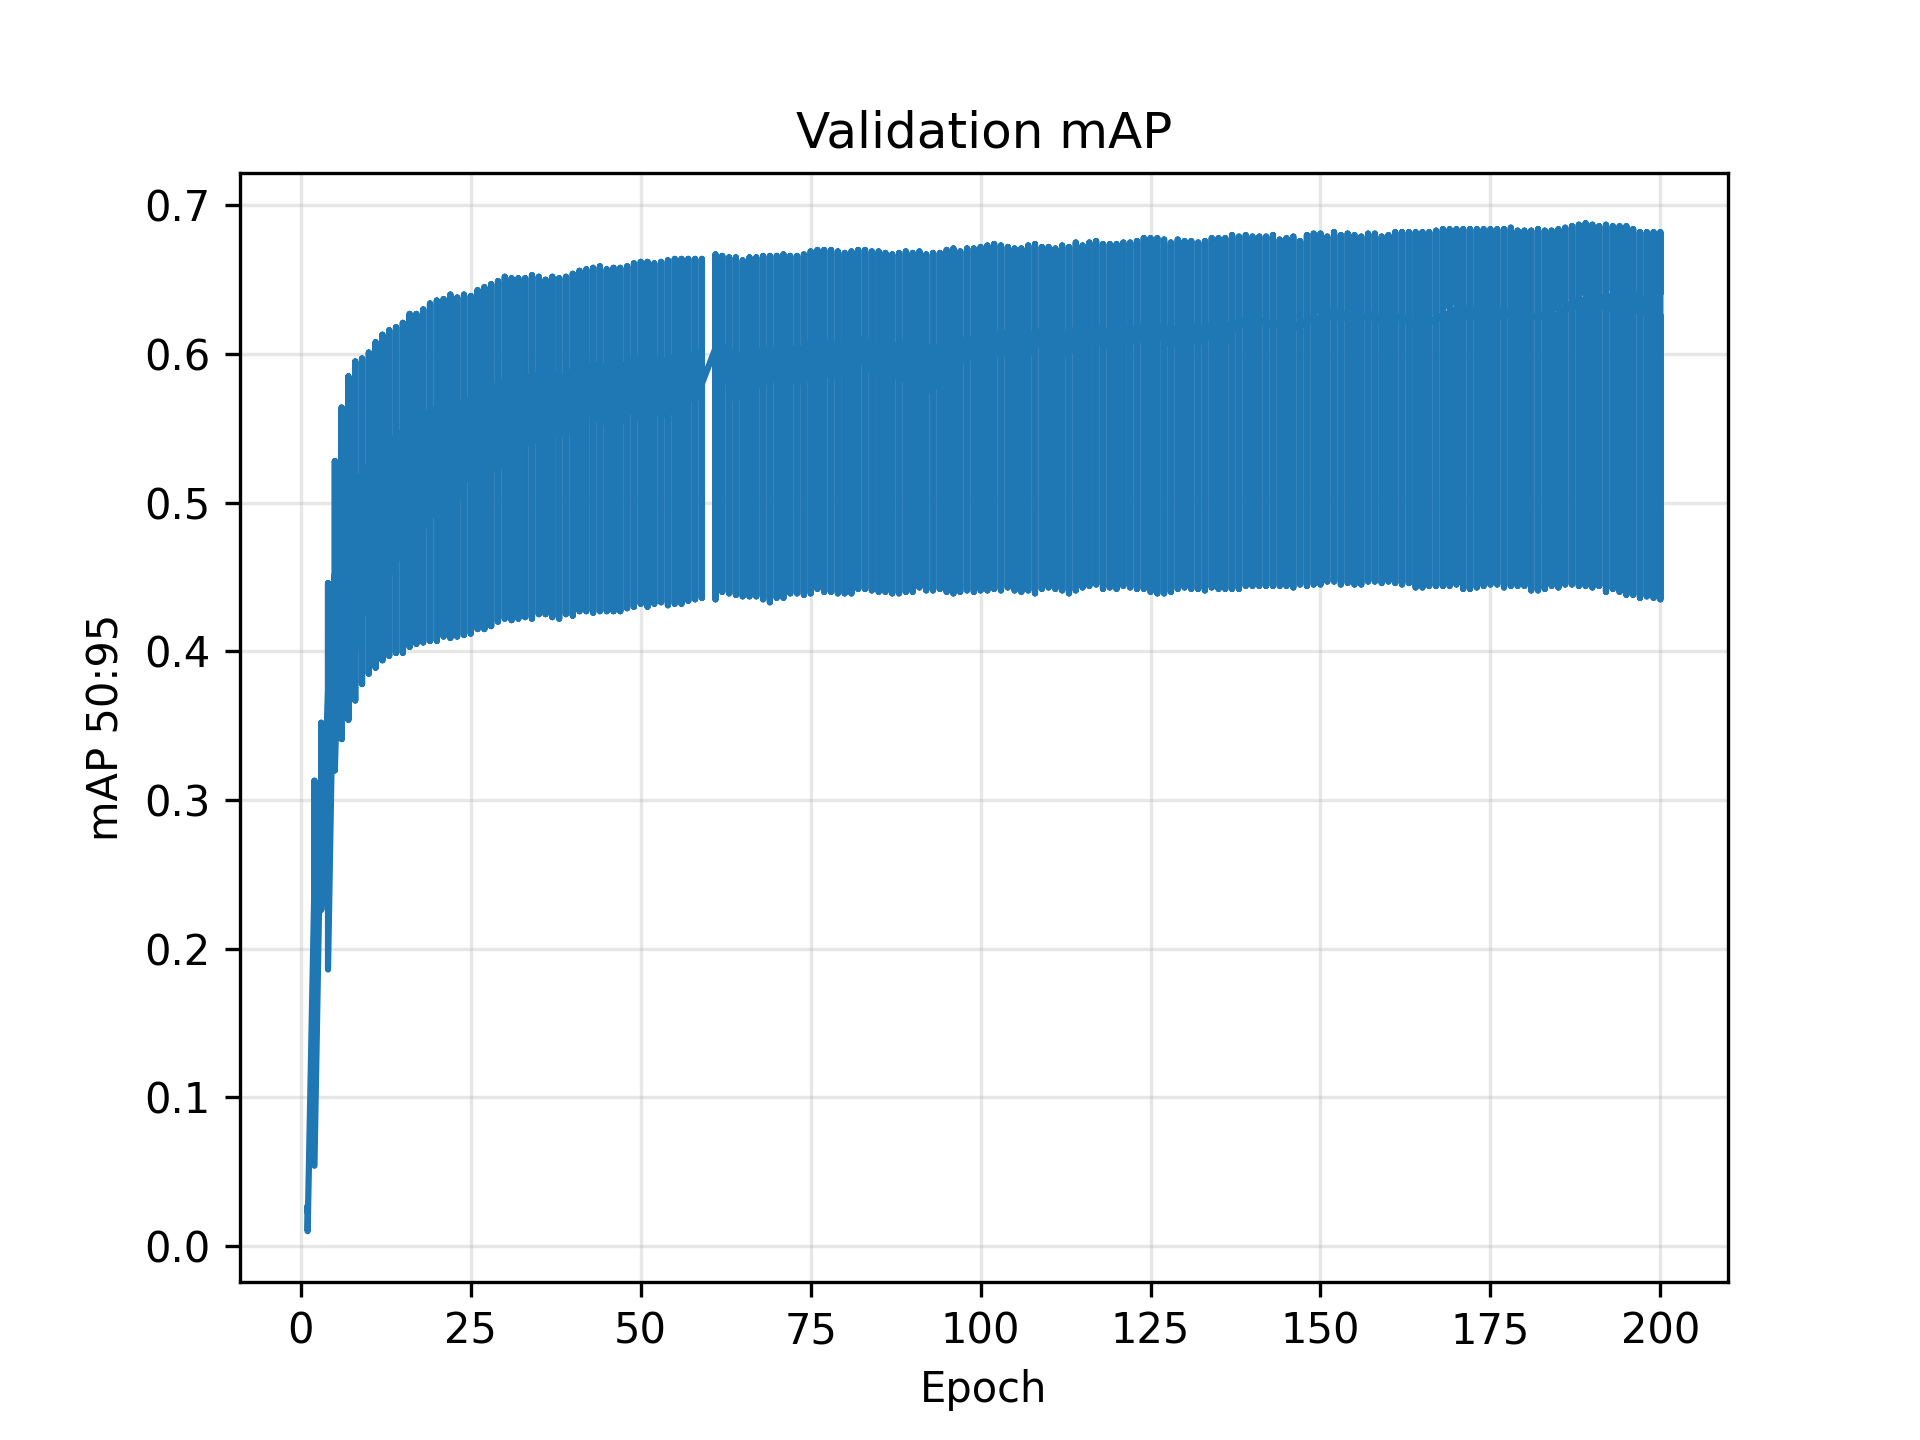
\includegraphics[width=\linewidth]{figures/images/chapter-11/licenseplate/v0/map_curve.png}
\caption{Validation mAP}
\end{subfigure}

\vspace{0.4cm}

\begin{subfigure}{0.50\textwidth}
\centering
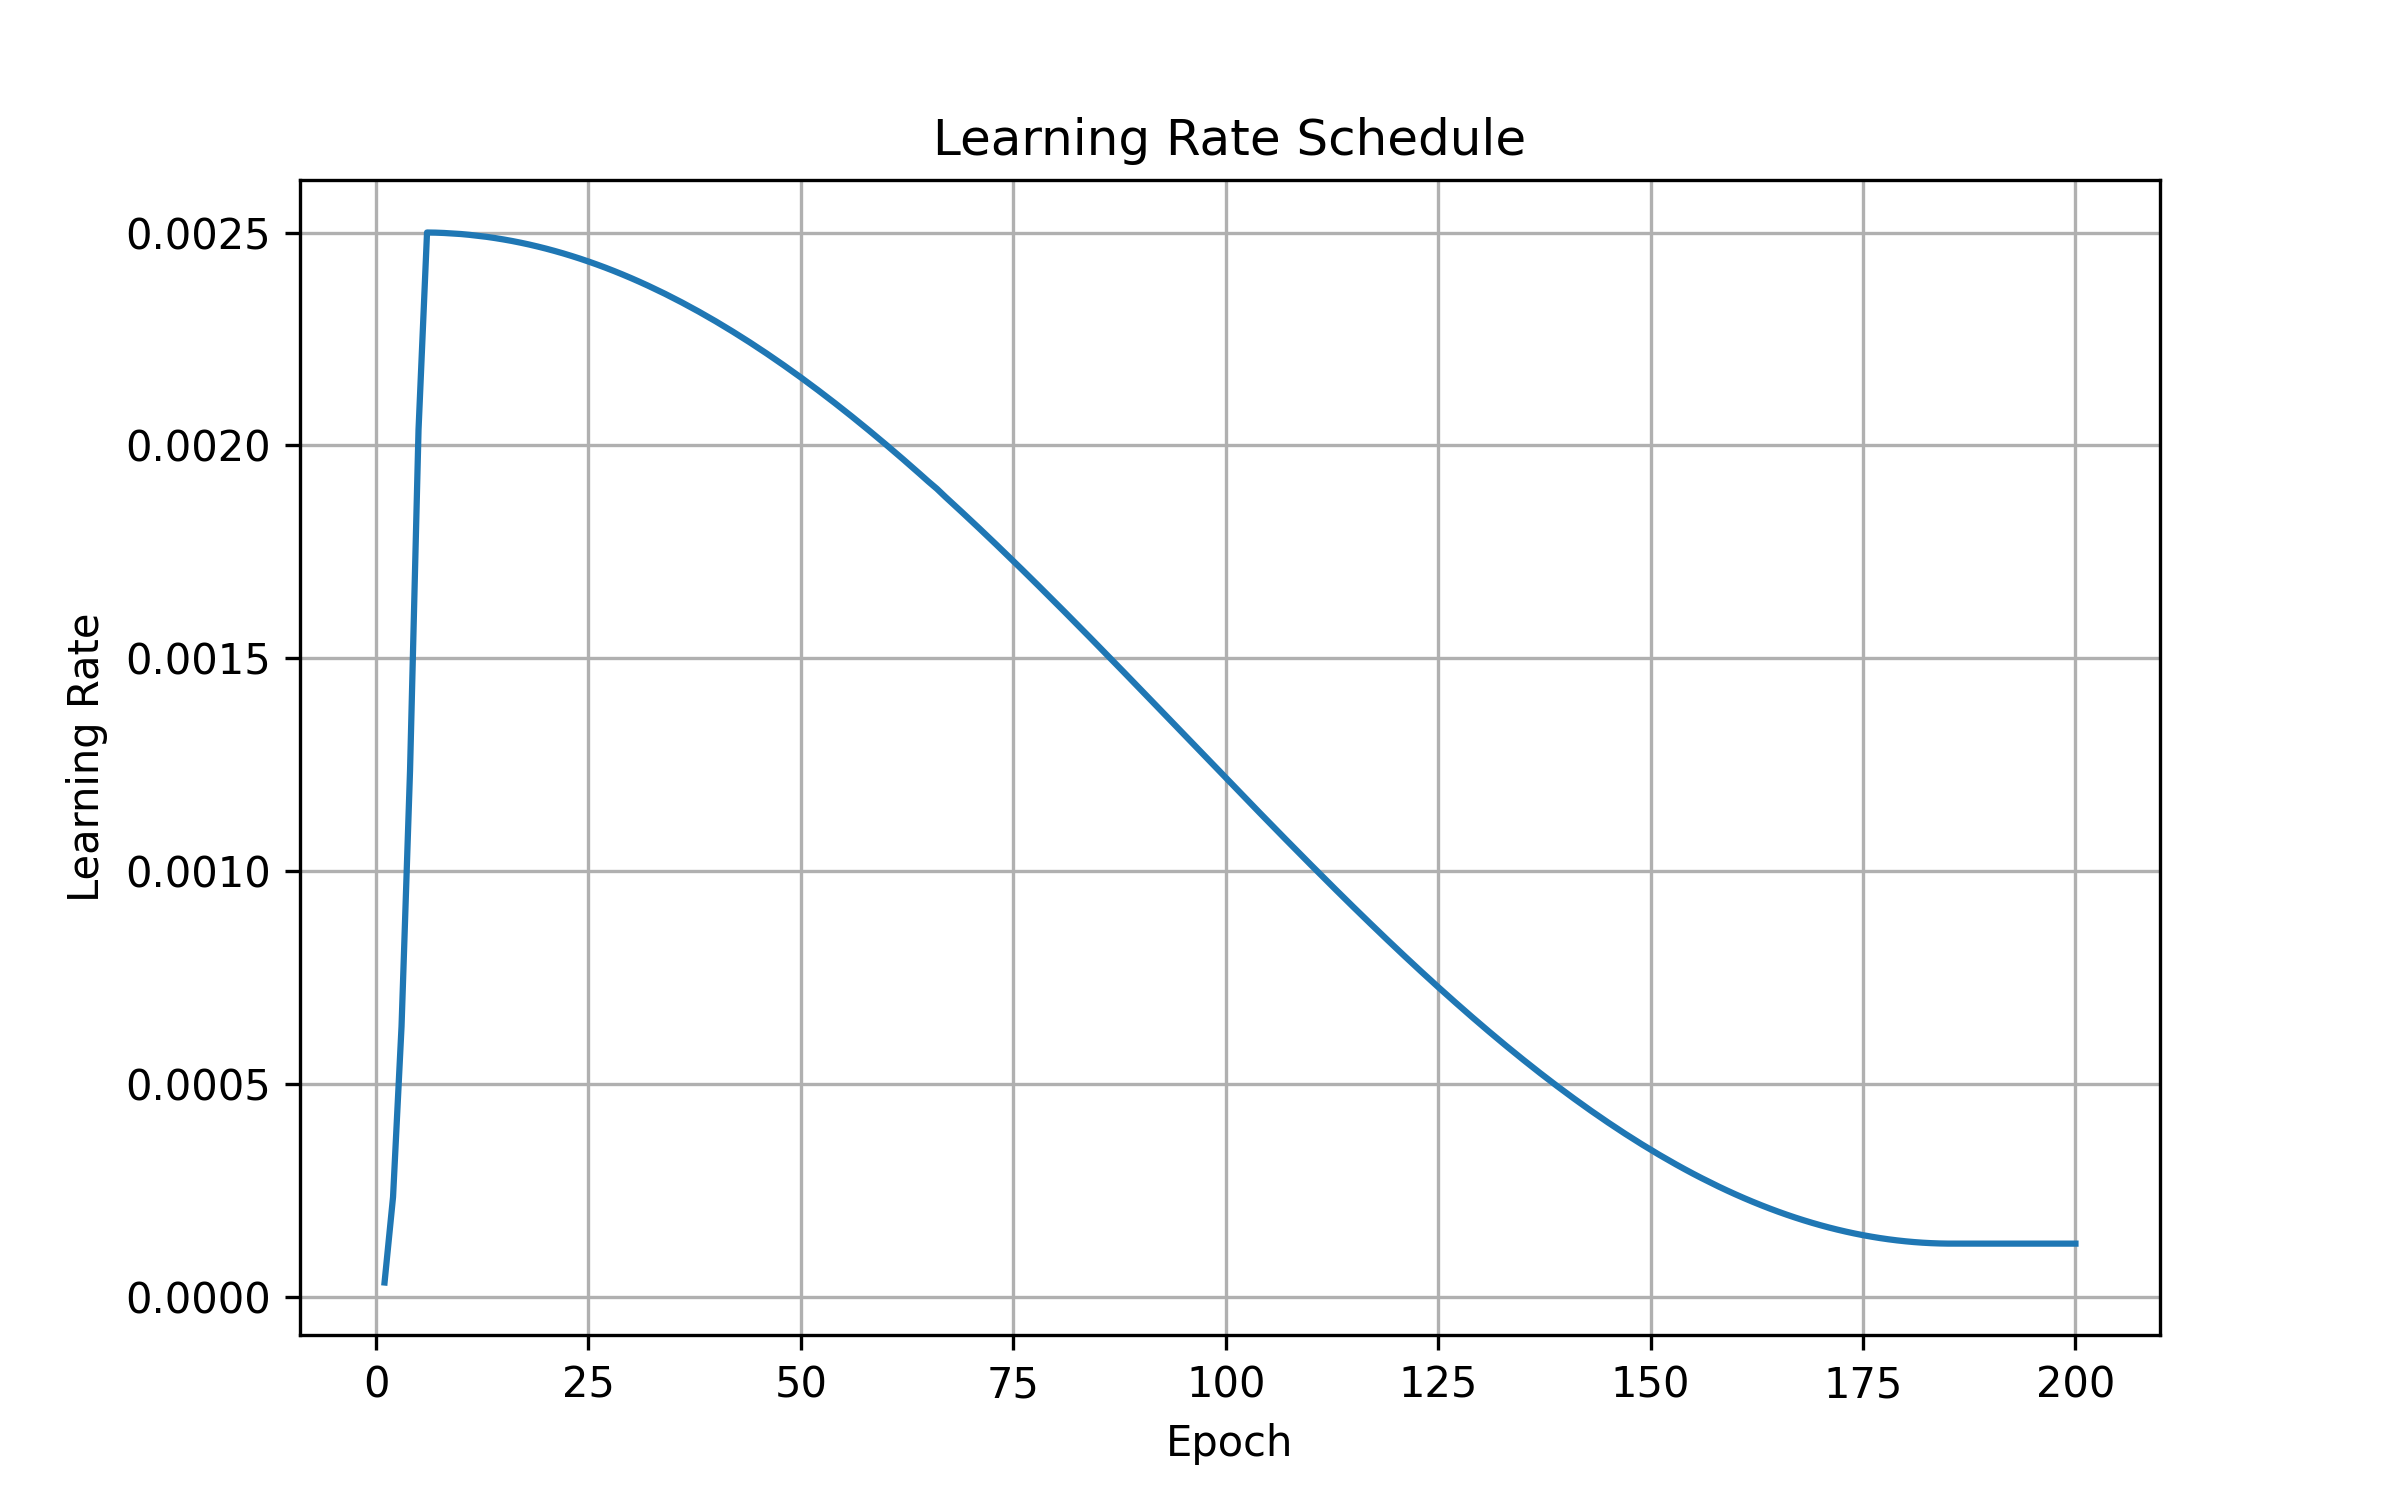
\includegraphics[width=\linewidth]{figures/images/chapter-11/licenseplate/v0/lr_curve.png}
\caption{Learning rate schedule}
\end{subfigure}

\caption{Training behaviour of model v0.}
\label{fig:lp_training_v0}

\end{figure}

\begin{figure}[H]
\centering

\begin{subfigure}{0.50\textwidth}
\centering
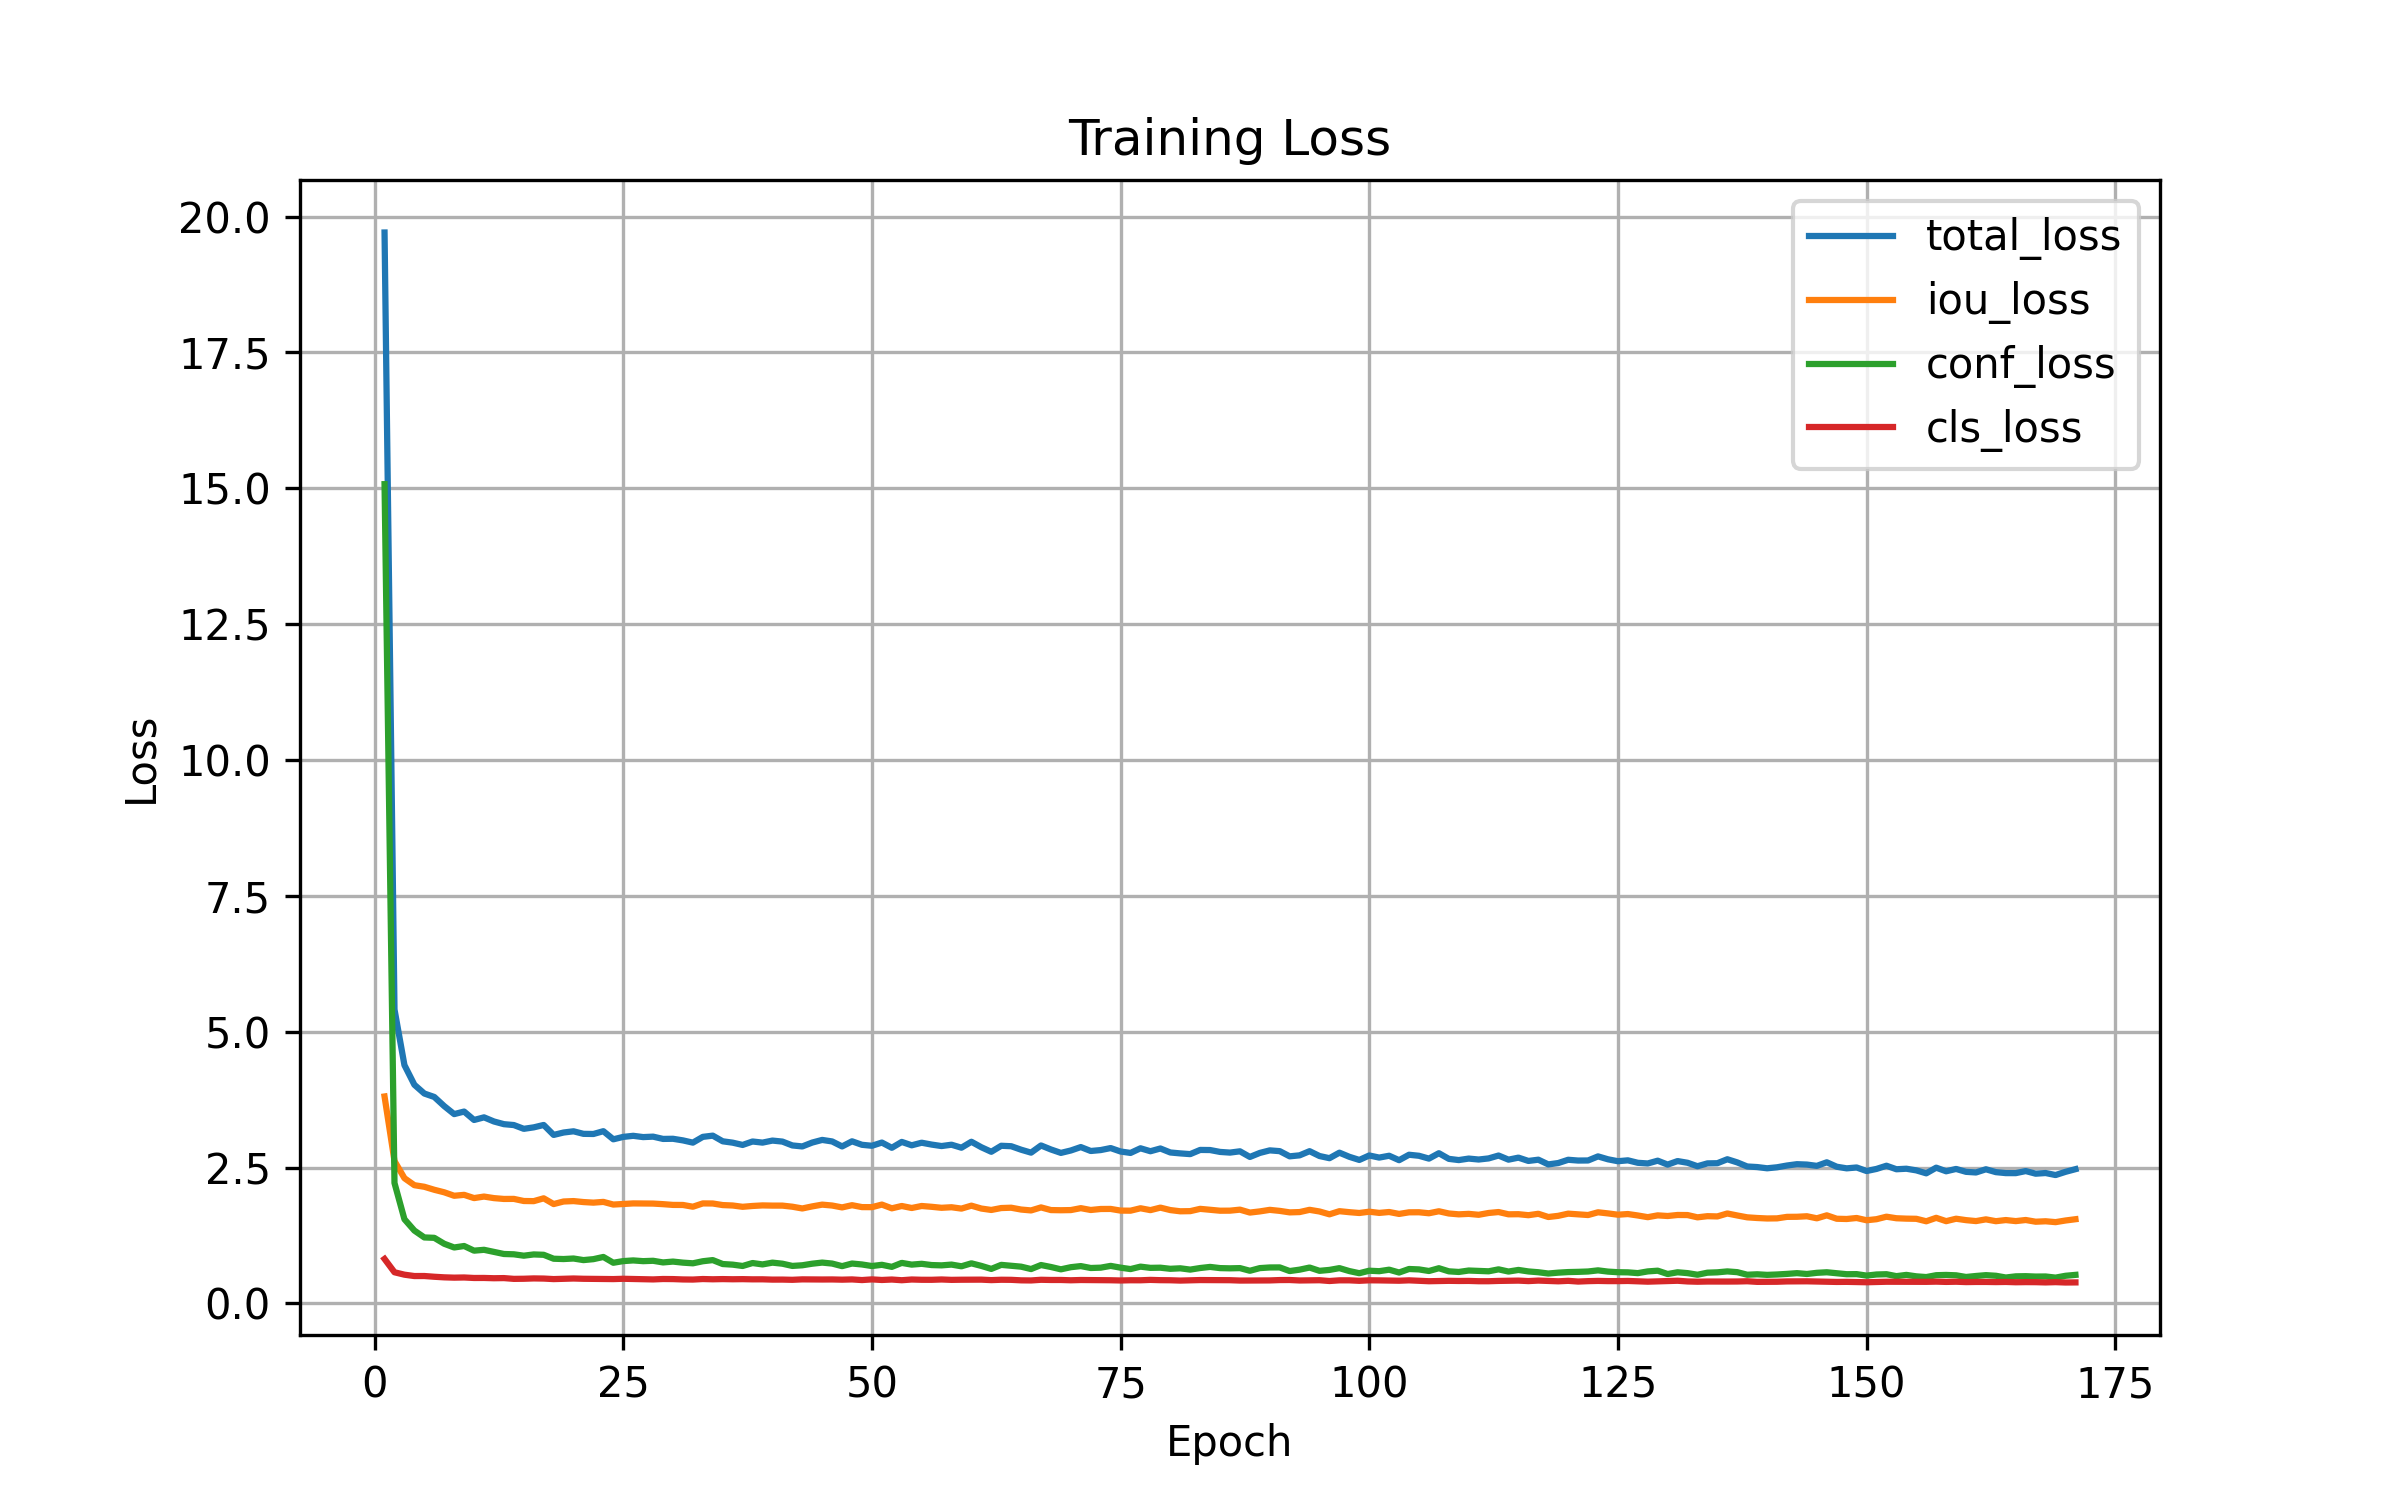
\includegraphics[width=\linewidth]{figures/images/chapter-11/licenseplate/v1/loss_curve.png}
\caption{Training loss}
\end{subfigure}
\hfill
\begin{subfigure}{0.48\textwidth}
\centering
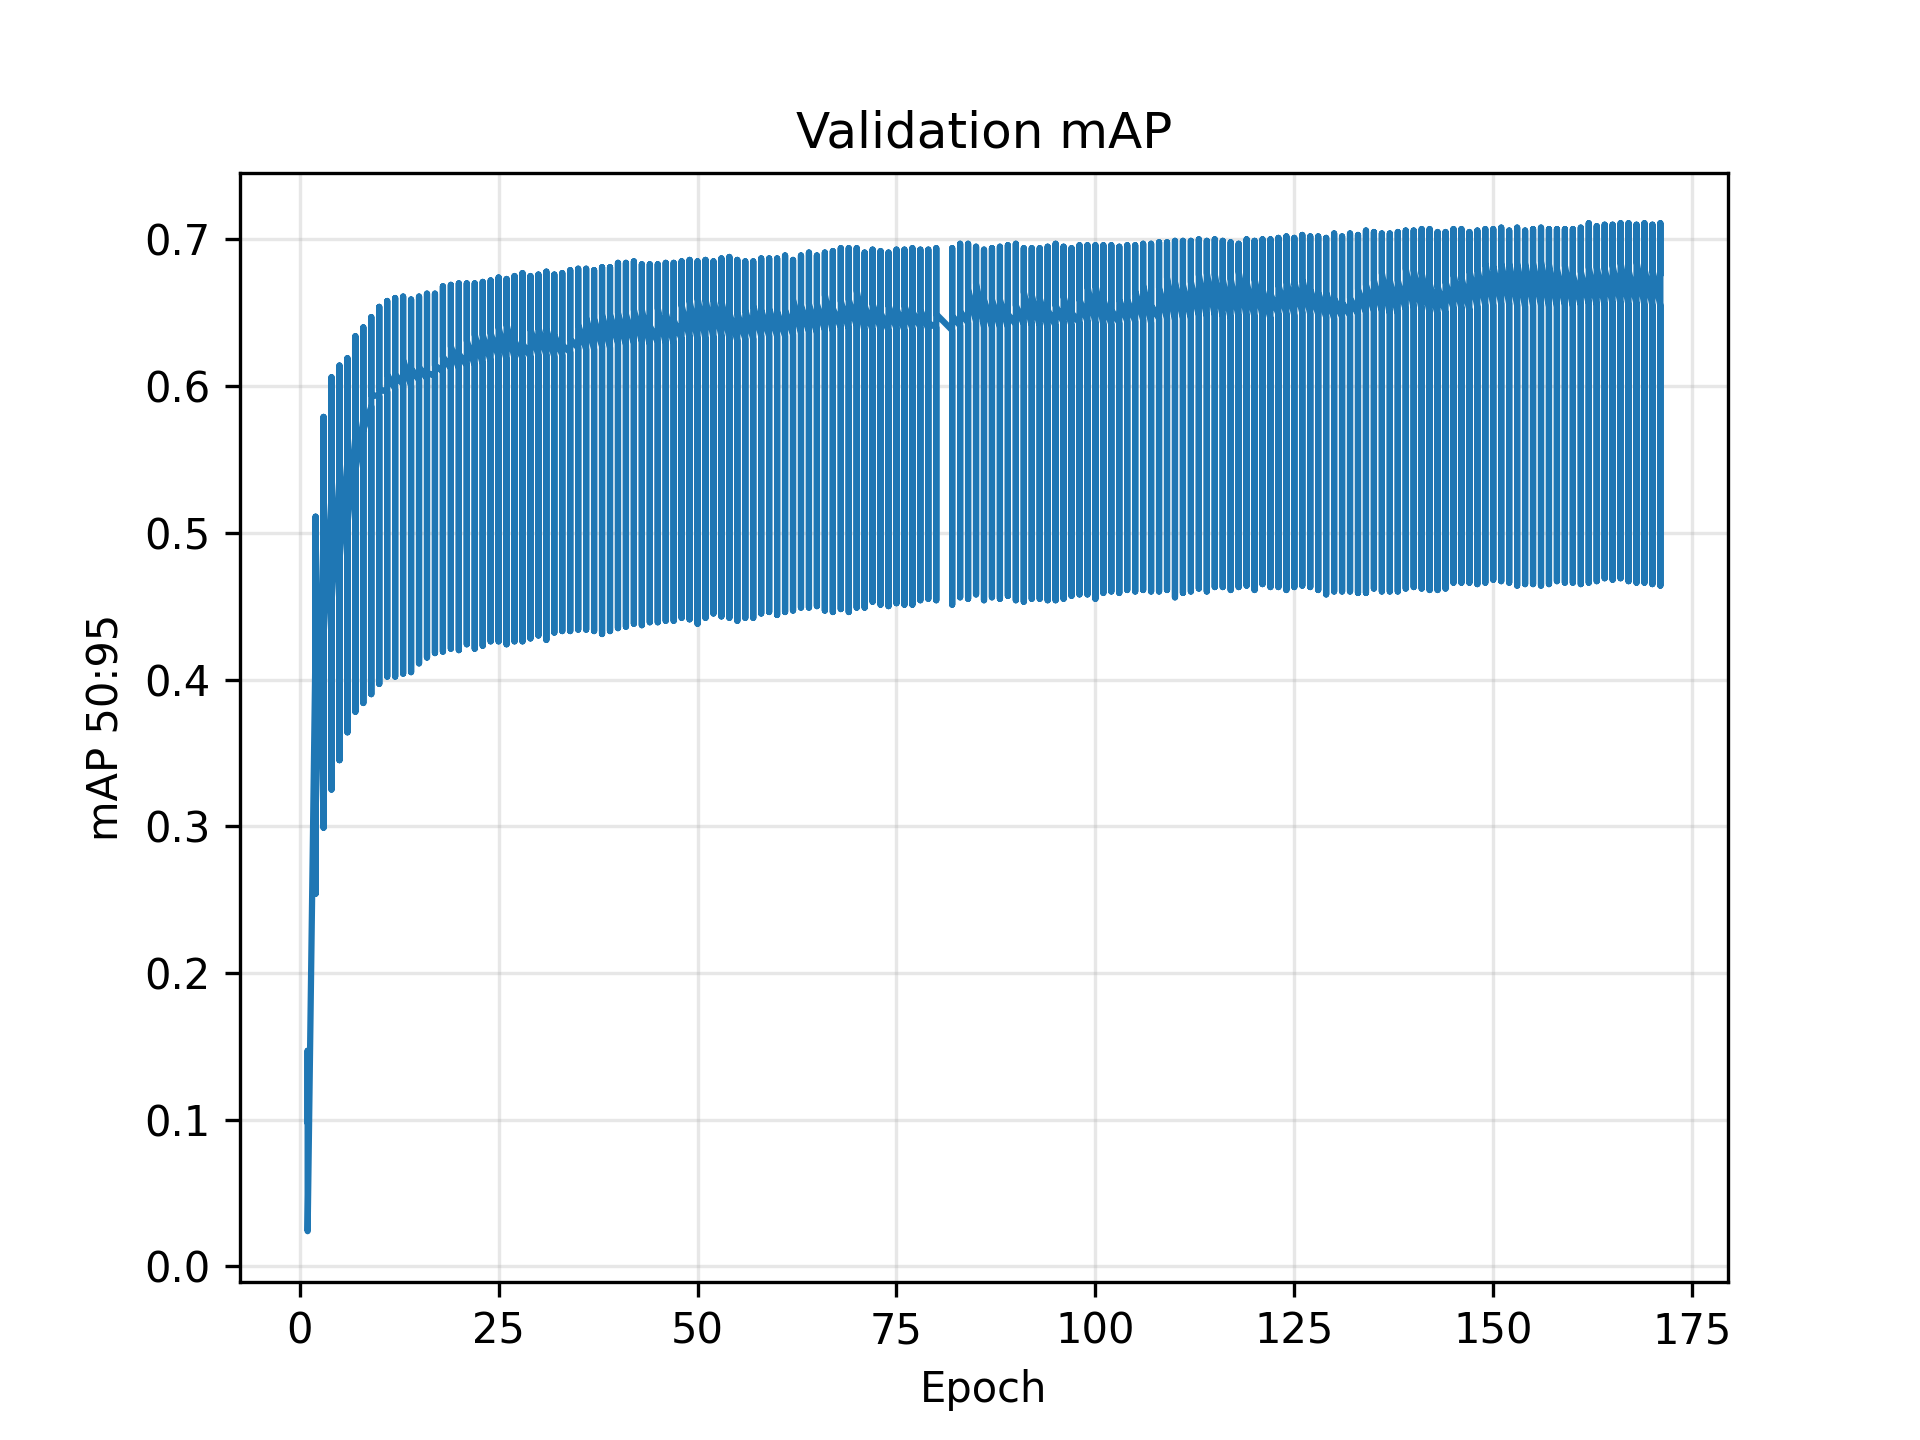
\includegraphics[width=\linewidth]{figures/images/chapter-11/licenseplate/v1/map_curve.png}
\caption{Validation mAP}
\end{subfigure}

\vspace{0.4cm}

\begin{subfigure}{0.50\textwidth}
\centering
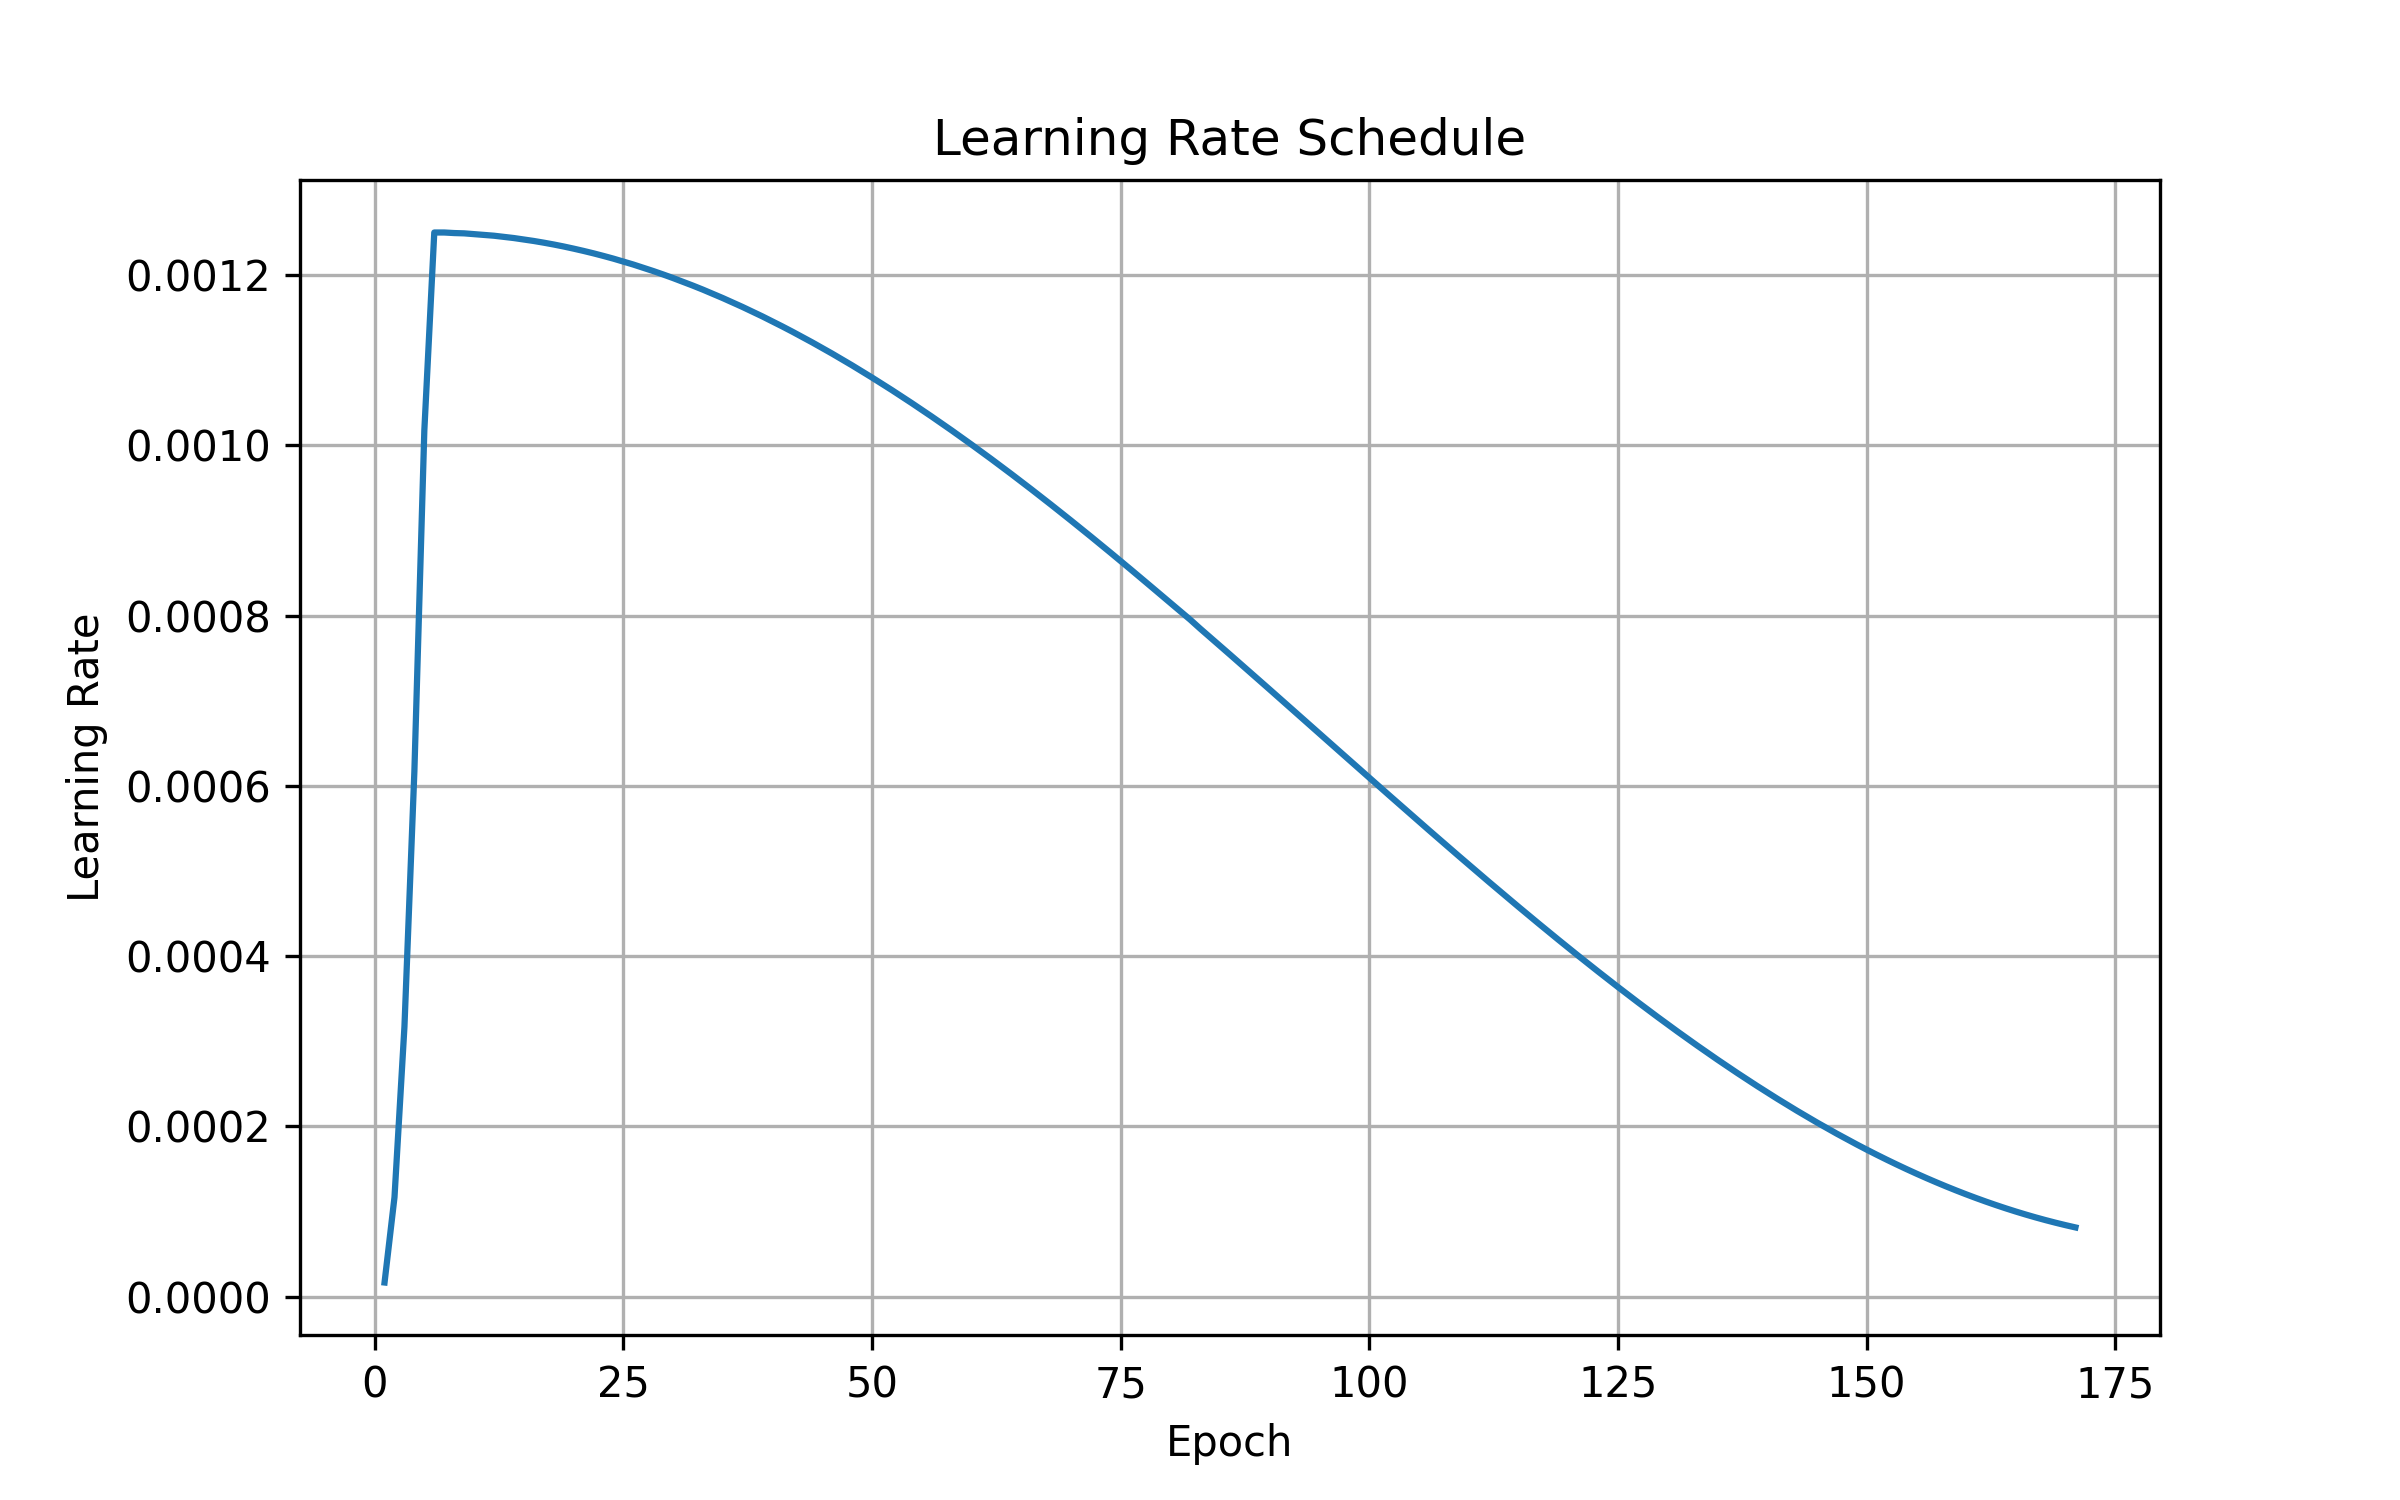
\includegraphics[width=\linewidth]{figures/images/chapter-11/licenseplate/v1/lr_curve.png}
\caption{Learning rate schedule}
\end{subfigure}

\caption{Training behaviour of model v1.}
\label{fig:lp_training_v1}

\end{figure}

Figure~\ref{fig:lp_training_v0} and Figure~\ref{fig:lp_training_v1} show the
training behaviour of the two license plate detection models. For both models,
the training loss decreases rapidly during the first epochs and then gradually
stabilizes, indicating stable optimization.

The validation mAP increases quickly at the beginning of training and then
continues to improve more gradually. Model v0 was trained for the full 200
epochs, while model v1 stopped earlier at approximately 175 epochs due to the
early stopping criterion. In both cases, the learning rate follows the expected
warm-up and decay schedule.







\subsection{Precision--Recall Analysis}

\begin{figure}[H]
\centering

\begin{subfigure}{0.48\textwidth}
\centering
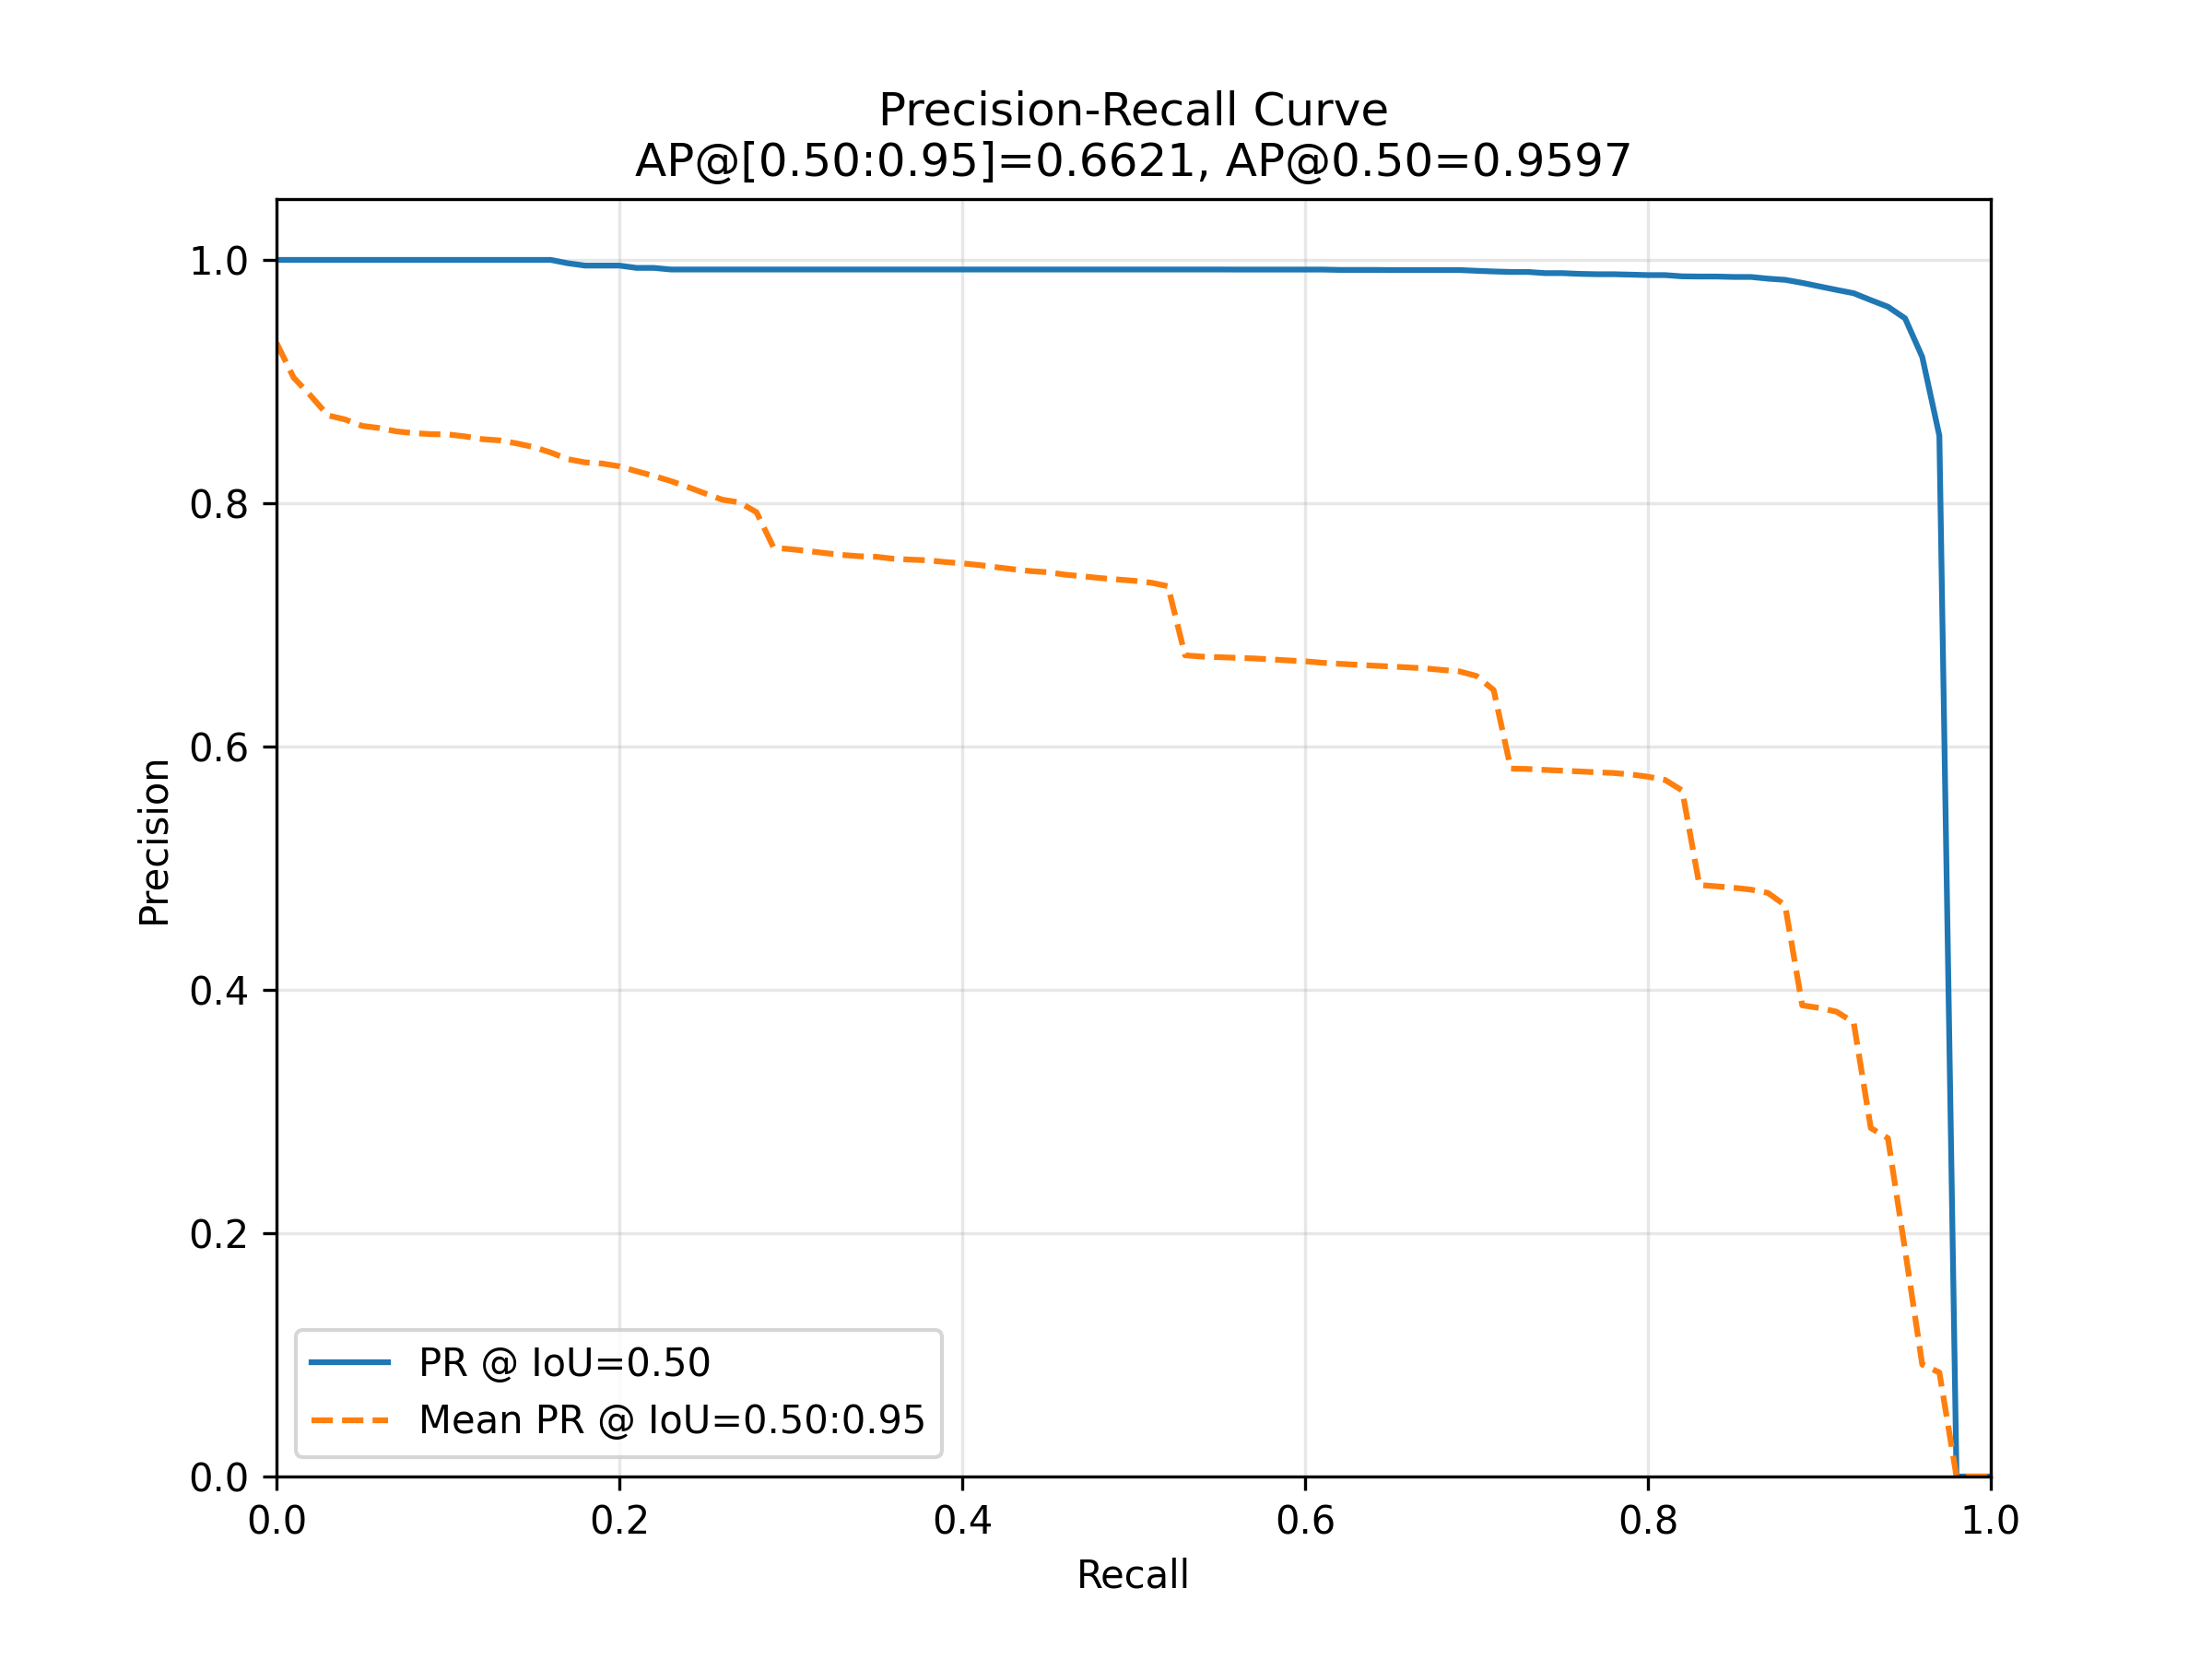
\includegraphics[width=\linewidth]{figures/images/chapter-11/licenseplate/v0/pr_curve.png}
\caption{V0 configuration.}
\end{subfigure}
\hfill
\begin{subfigure}{0.48\textwidth}
\centering
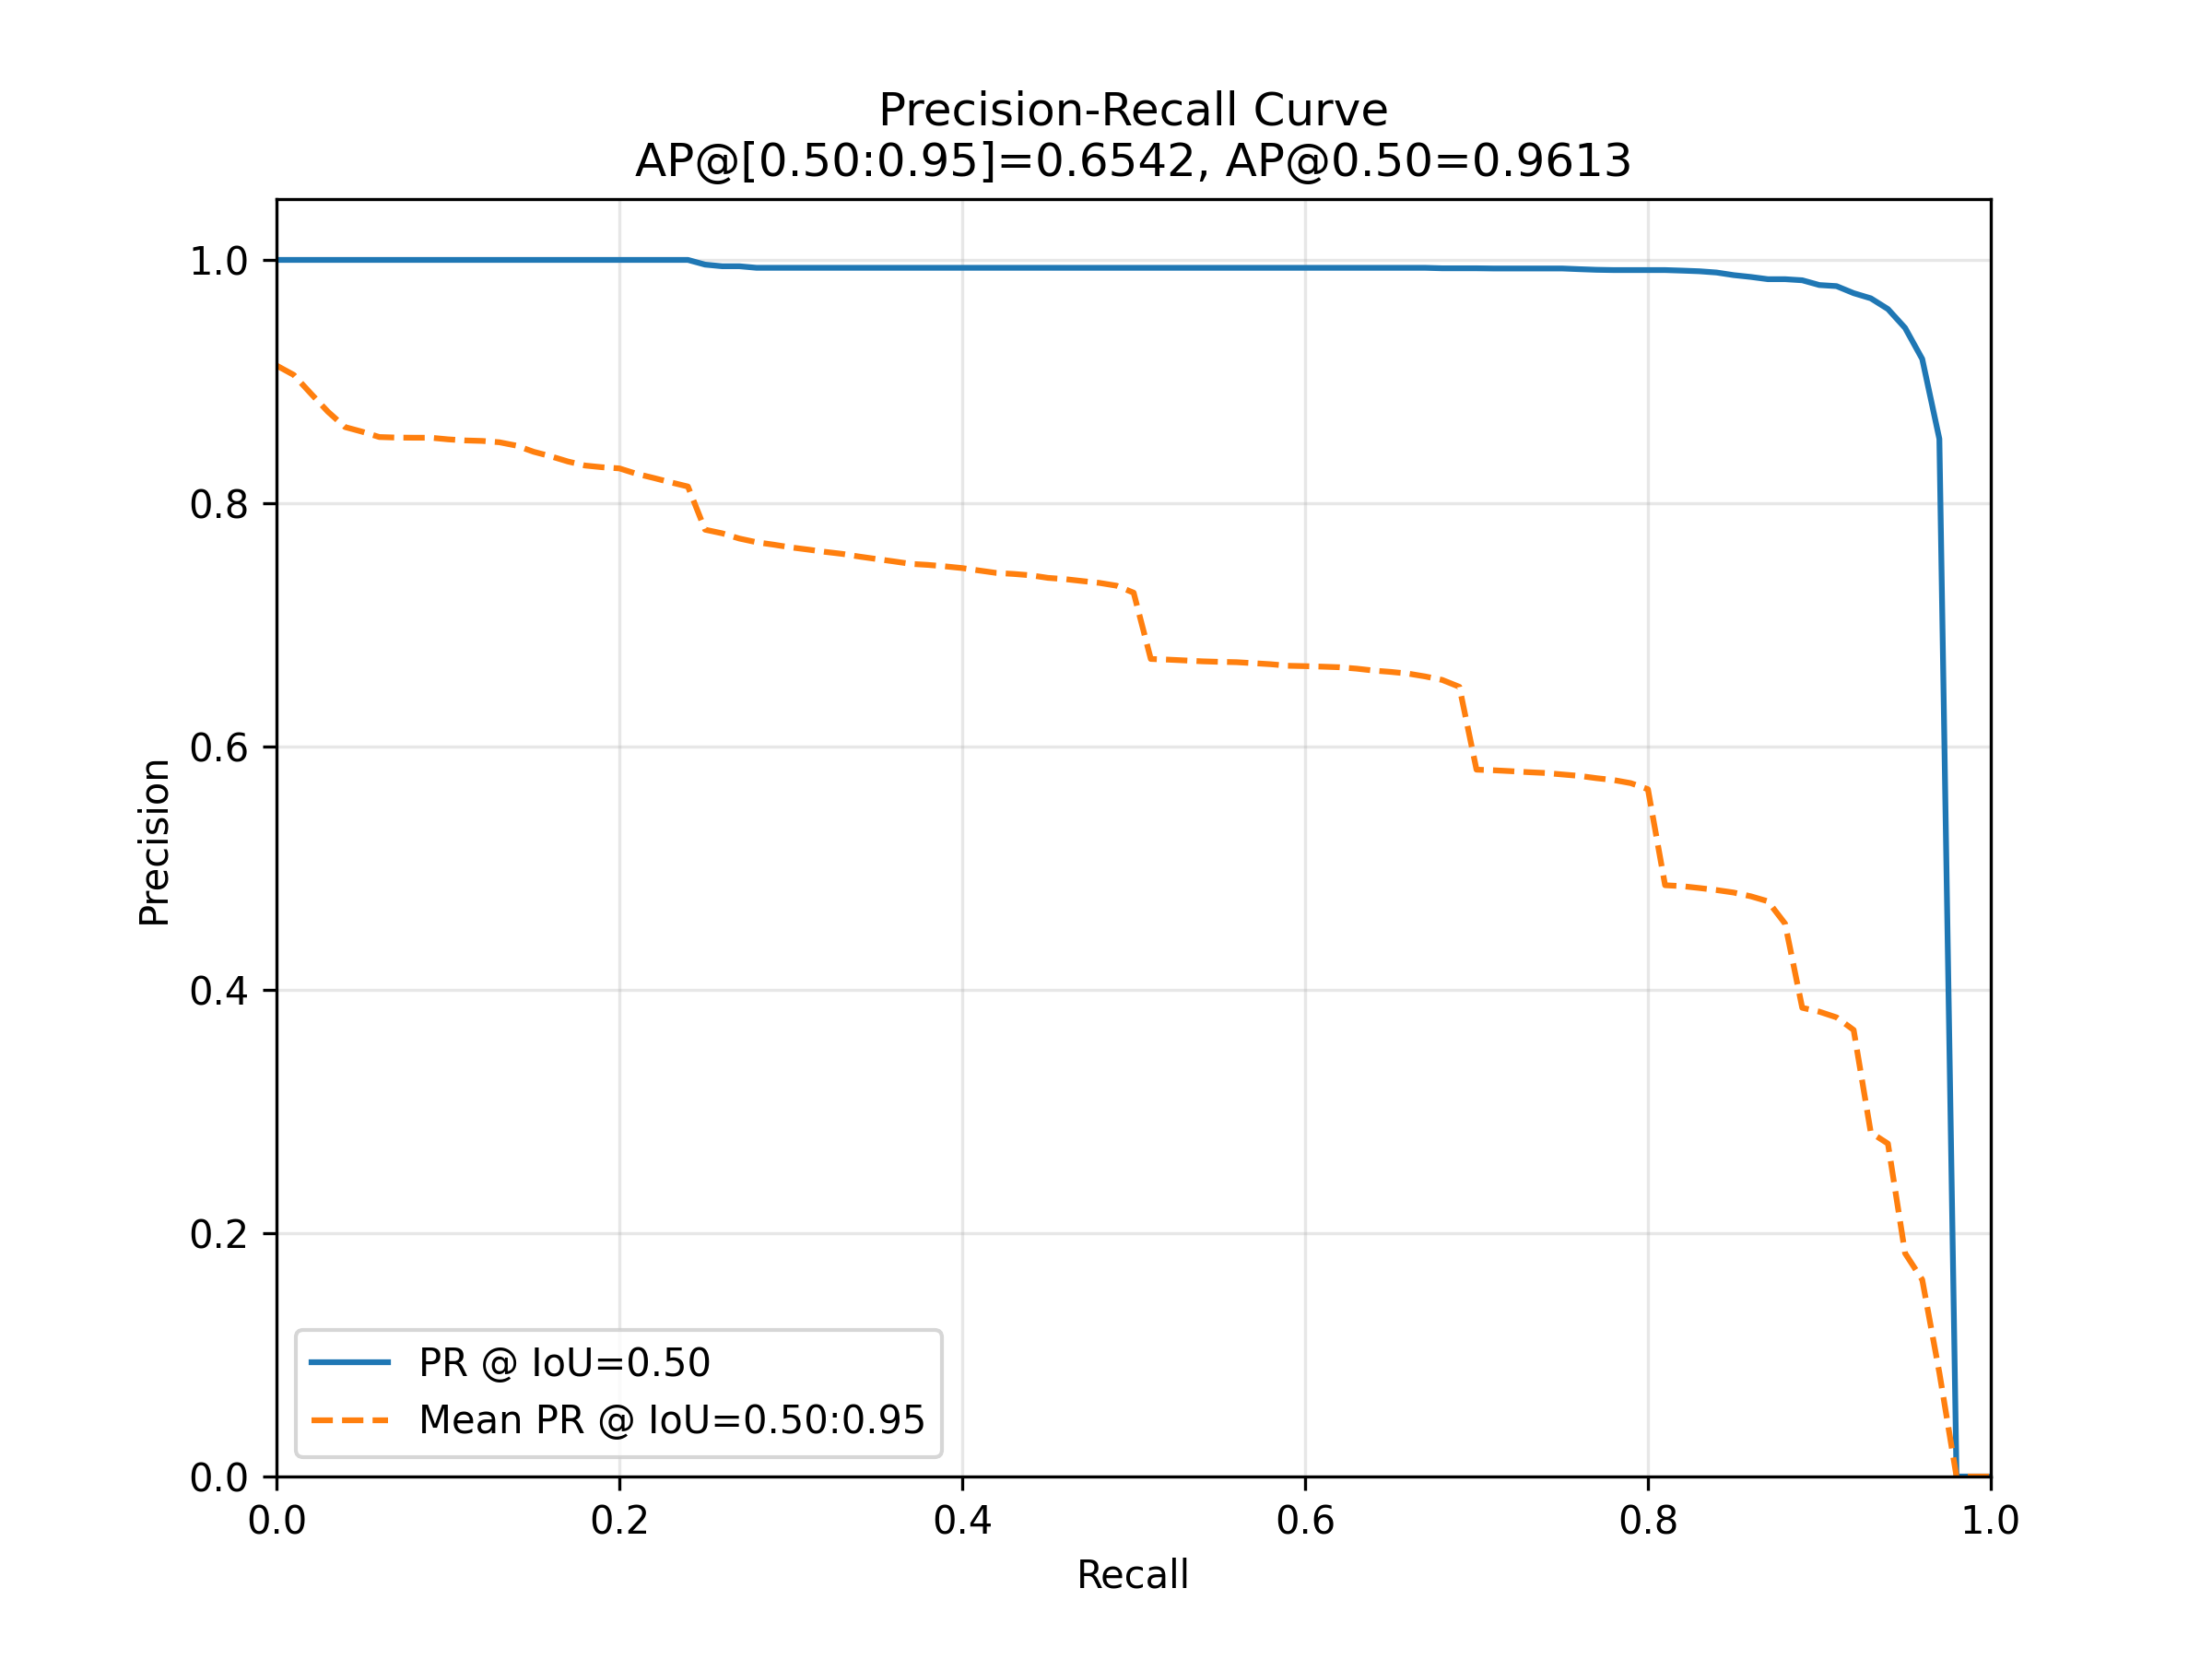
\includegraphics[width=\linewidth]{figures/images/chapter-11/licenseplate/v1/pr_curve.png}
\caption{V1 configuration.}
\end{subfigure}

\caption{Side-by-side comparison of the precision--recall curves for the v0 and v1 configurations.}
\label{fig:lp_pr_curves_licenseplate} 
\end{figure}

Figure~\ref{fig:lp_pr_curves_licenseplate} shows the precision--recall curves for the two
license plate detection models. Both configurations achieve a high AP@0.50,
with v0 reaching 0.9597 and v1 reaching 0.9613. This indicates strong detection
performance for both models at an IoU threshold of 0.50.

The AP@0.50:0.95 values are also similar, with v0 achieving 0.6621 and v1
achieving 0.6542. Although v1 performs slightly better at AP@0.50, v0 obtains a
slightly higher score across the stricter IoU range. Overall, the
precision--recall analysis shows that the two configurations perform similarly,
with only small differences between them.





\subsection{Confusion Matrix Analysis}

\begin{figure}[H]
\centering
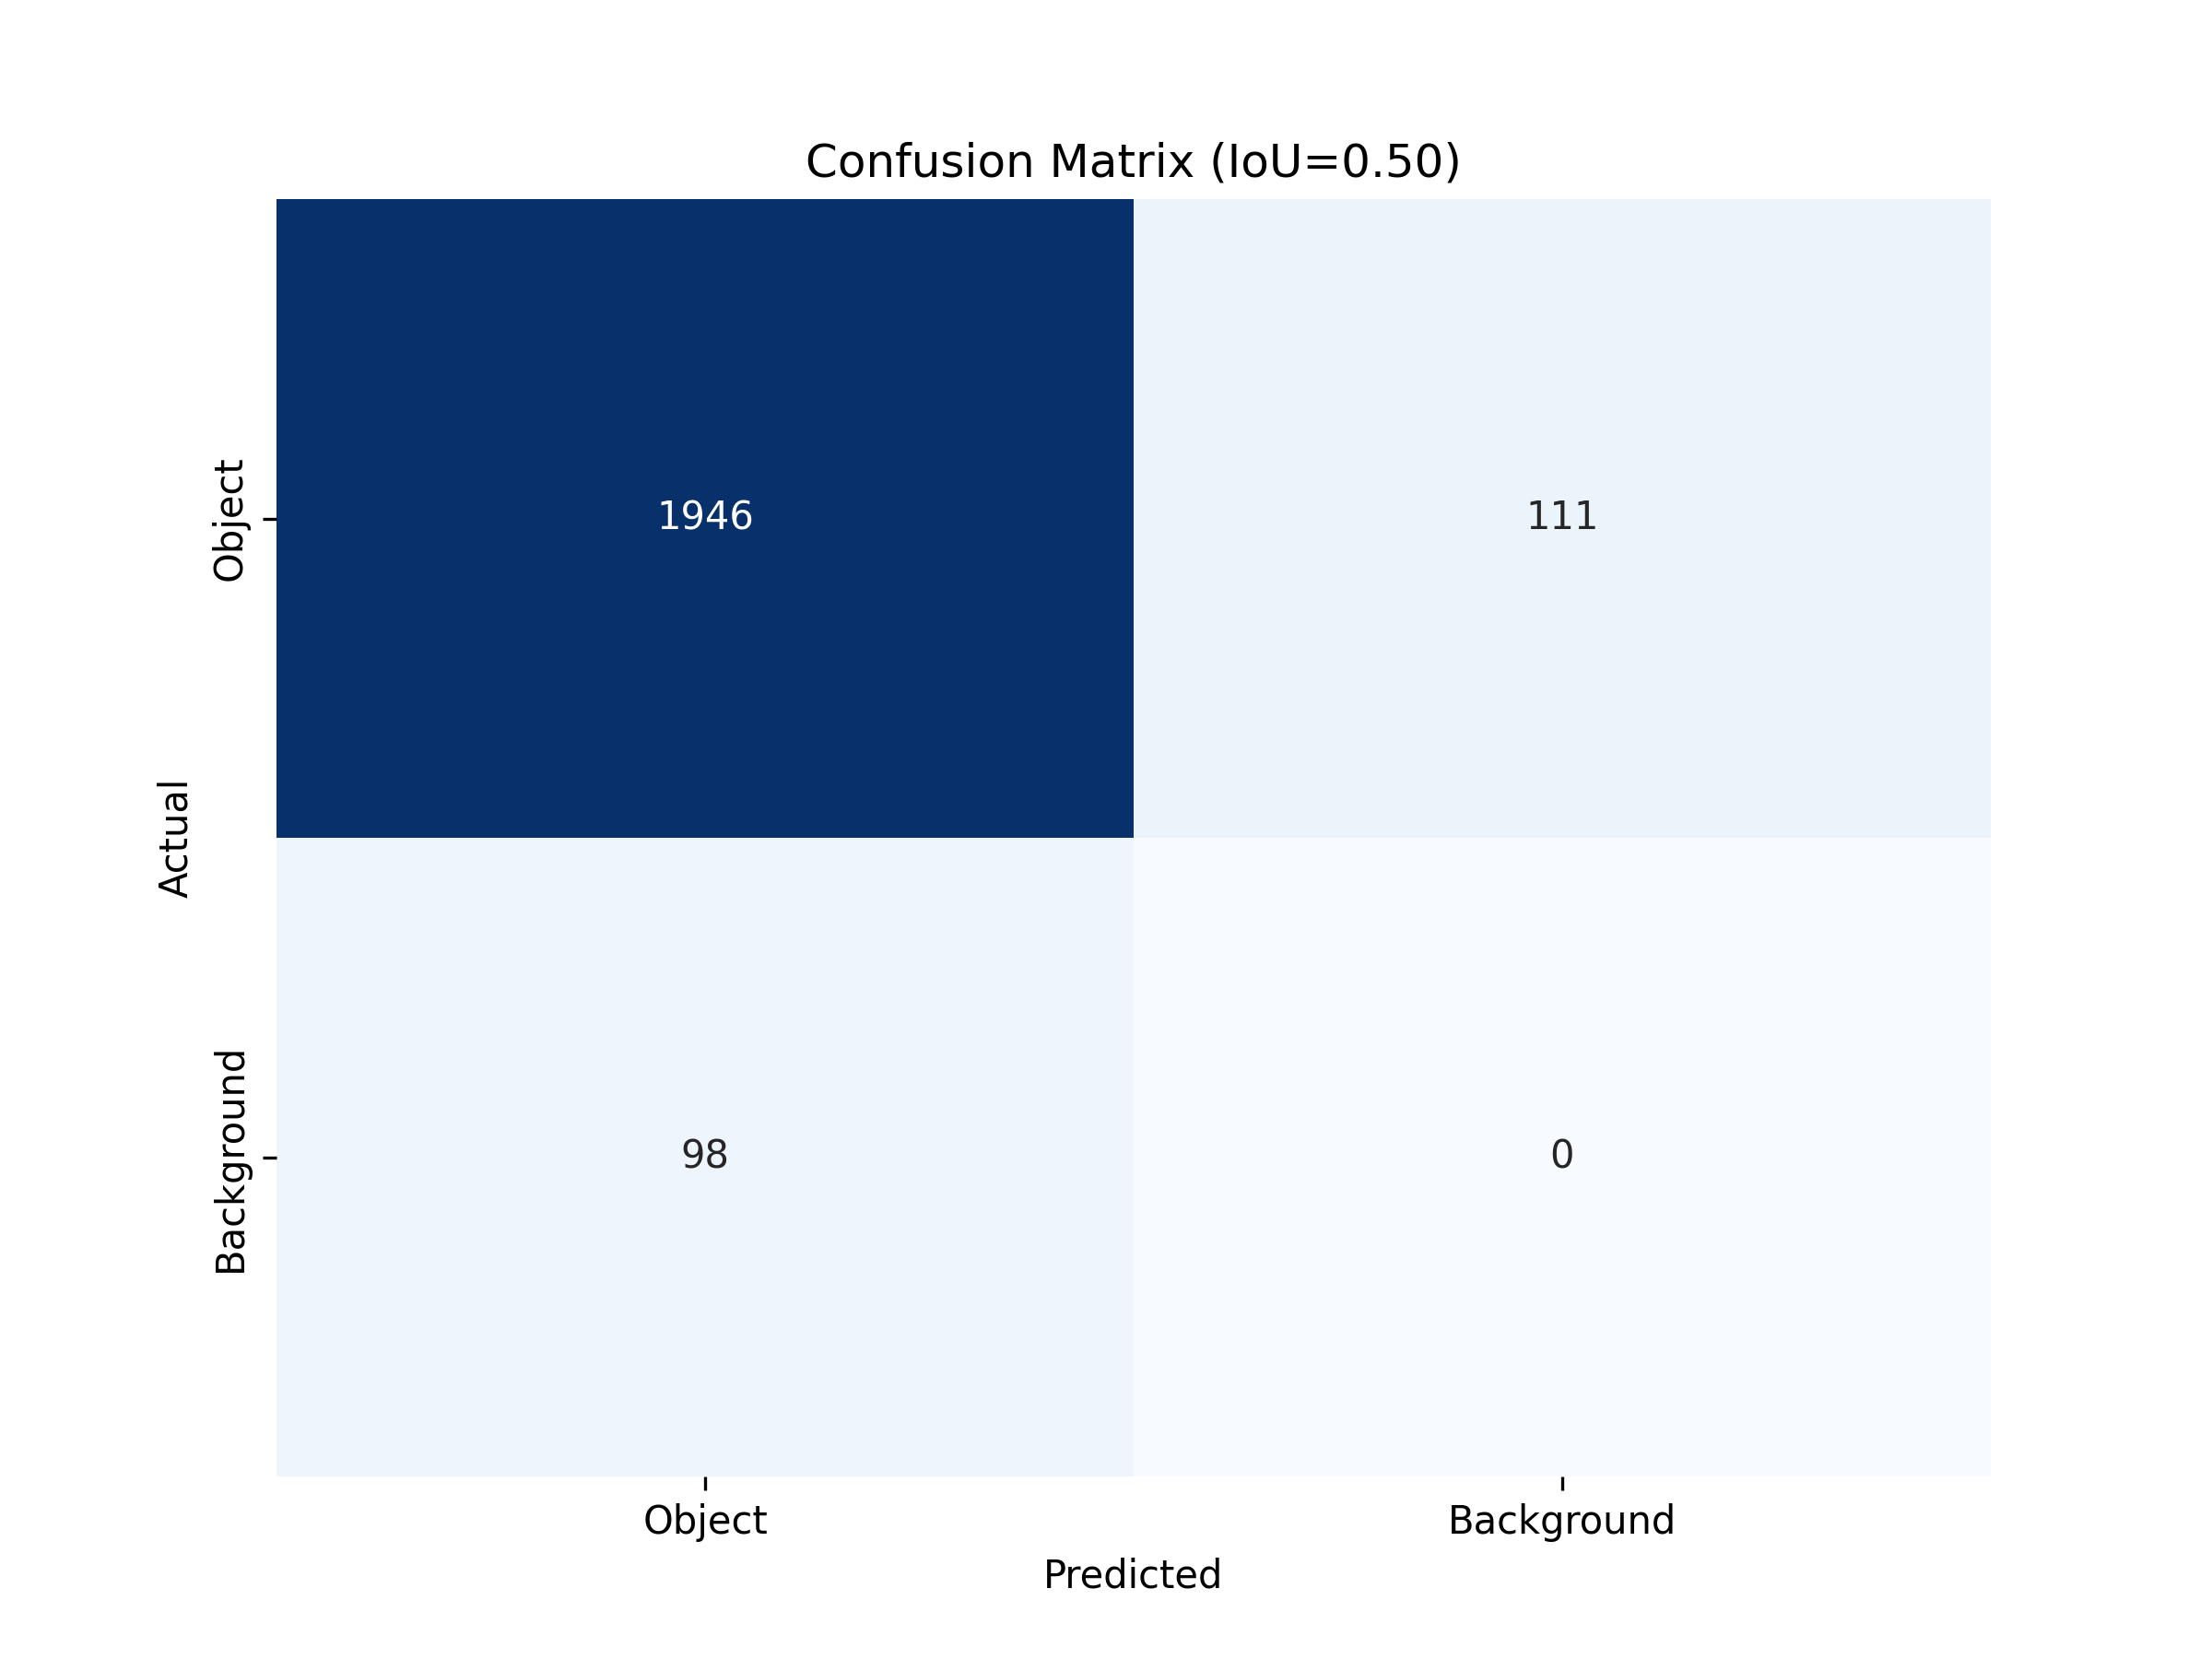
\includegraphics[width=12cm]{figures/images/chapter-11/licenseplate/v0/confusion_matrix_0.3.png}
\caption{Confusion matrix for the v0 configuration.}
\label{fig:lp_confusion_matrix_v0}
\end{figure}

\begin{figure}[H]
\centering
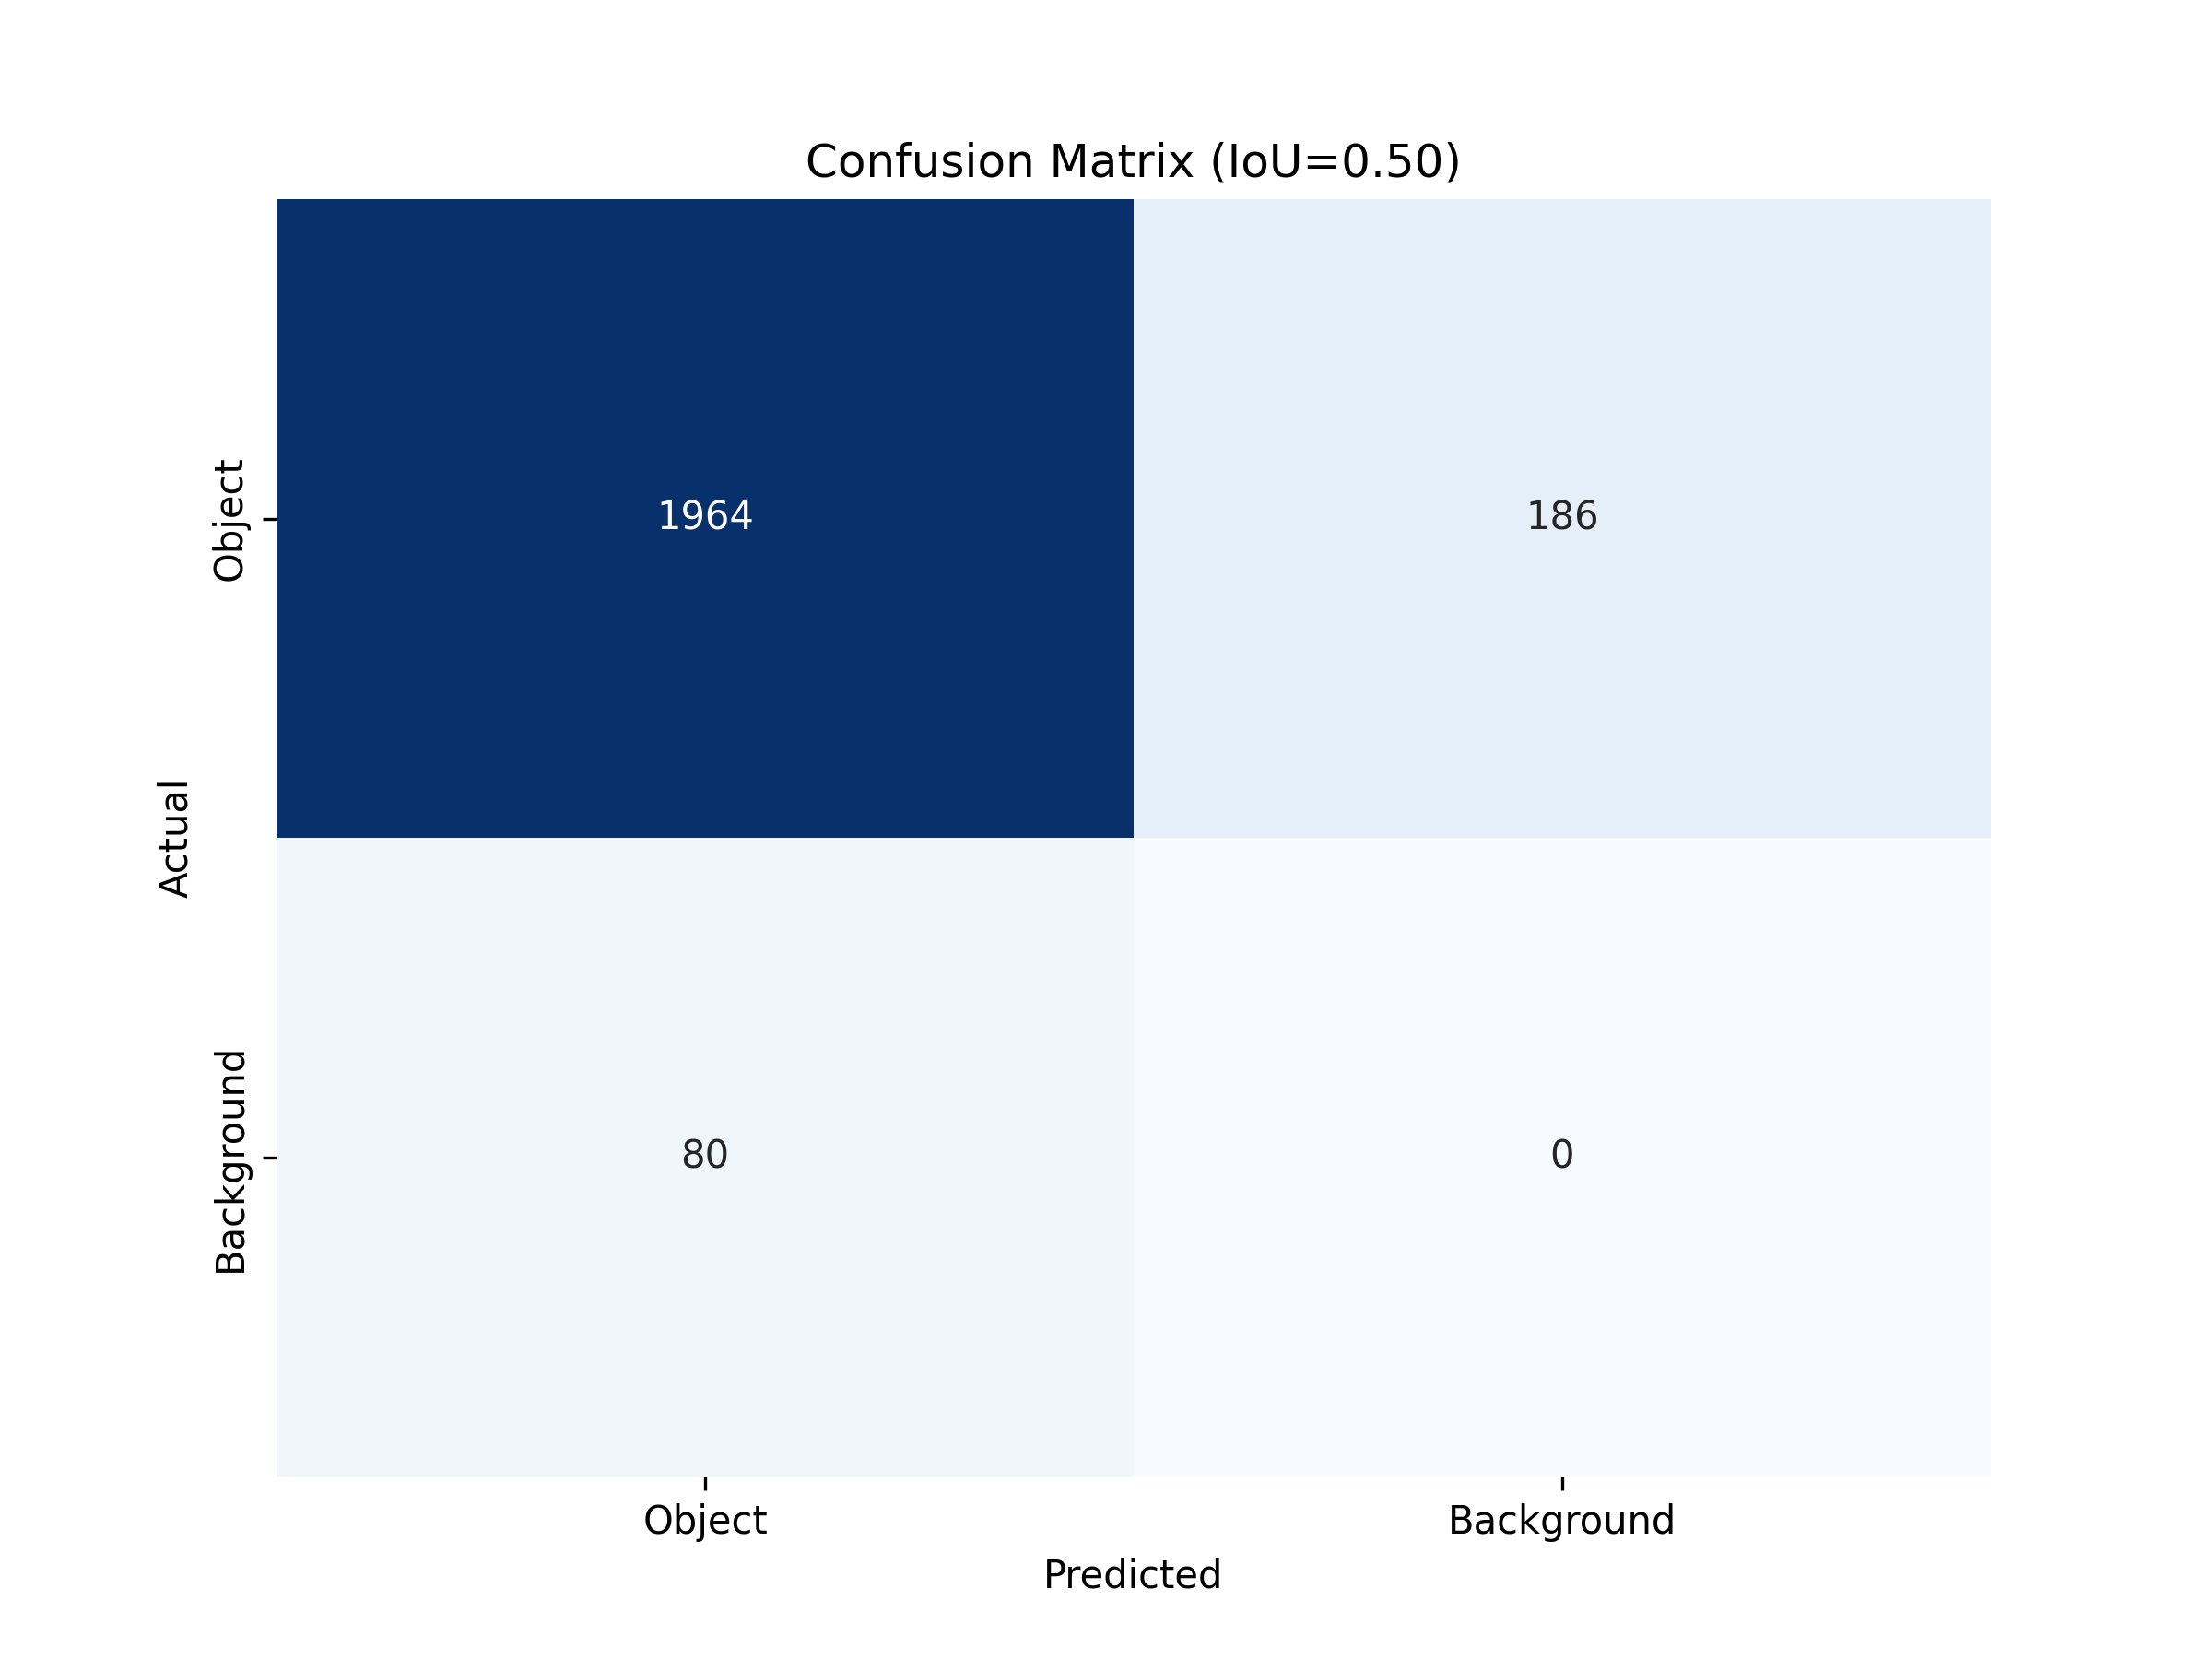
\includegraphics[width=12cm]{figures/images/chapter-11/licenseplate/v1/confusion_matrix_0.3.png}
\caption{Confusion matrix for the v1 configuration.}
\label{fig:lp_confusion_matrix_v1}
\end{figure}

Figure~\ref{fig:lp_confusion_matrix_v0} and
Figure~\ref{fig:lp_confusion_matrix_v1} show the confusion matrices for the two
license plate detection models at an IoU threshold of 0.50.

The confusion matrix values do not directly match the number of test images
because object detection is evaluated at the object level. Each image may
contain multiple license plates and multiple predicted bounding boxes.
Therefore, the matrix counts detections and missed objects rather than images.

The F1-score was calculated as the harmonic mean of precision and recall:
\[
F1 = 2 \cdot \frac{Precision \cdot Recall}{Precision + Recall}
\]

The v0 configuration correctly detected 1946 license plates, produced 98 false
positive detections, and missed 111 license plates. This resulted in a
precision of 0.9521, a recall of 0.9460, and an F1-score of 0.9490.

The v1 configuration correctly detected 1964 license plates and produced fewer
false positives, with 80 false detections. However, it also missed more license
plates, with 186 false negatives. This resulted in a slightly higher precision
of 0.9609, but a lower recall of 0.9135 and an F1-score of 0.9366.

\begin{align*}
Precision_{v0} &= \frac{1946}{1946 + 98} \approx 0.9521,
&
Recall_{v0} &= \frac{1946}{1946 + 111} \approx 0.9460,
&
F1_{v0} &\approx 0.9490
\end{align*}

\begin{align*}
Precision_{v1} &= \frac{1964}{1964 + 80} \approx 0.9609,
&
Recall_{v1} &= \frac{1964}{1964 + 186} \approx 0.9135,
&
F1_{v1} &\approx 0.9366
\end{align*}

Overall, v1 is slightly more precise, while v0 achieves better recall and a
higher F1-score. This indicates that v0 provides a better balance between
detecting license plates and avoiding false detections.

\subsection{Summary}

Both license plate detection models achieved strong detection performance on
the unseen test set. Model v1 obtained slightly higher precision, while model
v0 achieved higher recall and a higher F1-score.

Since the proposed system benefits from detecting as many license plates as
possible while still maintaining high precision, the v0 configuration was
selected as the final license plate detection model. The results show that v0
provides the best overall balance between precision, recall, and F1-score. The final barcode detection model was therefore selected for use in the proposed system.










% --------------------------------------------------------------------------------


\section{Named Entity Recognition}
\label{app:ner_evaluation}

\subsection{Training Setup}

The NER model was trained as a token classification model based on XLM-RoBERTa. Unlike the barcode and license plate models, which were trained as object detectors, the NER component addressed sequence labeling of \acrshort{ocr} extracted text. The training workflow combined synthetically generated data with converted external NER datasets in order to balance \acrshort{ocr} specific privacy entities with more natural running-text examples.

\begin{table}[H]
\centering
\begin{tabular}{l r}
\toprule
\textbf{Dataset source} & \textbf{Samples} \\
\midrule
Synthetic dataset & 199000 \\
NorNE (converted) \cite{norne_sprakbanken} & 15000 \\
English NER dataset (converted) \cite{kaggle_ner_dataset} & 15000 \\
\midrule
Total merged dataset & 229000 \\
\bottomrule
\end{tabular}
\caption{Composition of the merged NER dataset used before train/validation/test splitting.}
\label{tab:ner_dataset_composition}
\end{table}

\begin{table}[H]
\centering
\begin{tabular}{l r}
\toprule
\textbf{Split} & \textbf{Samples} \\
\midrule
Train & 183200 \\
Validation & 22900 \\
Test & 22900 \\
\bottomrule
\end{tabular}
\caption{Final split sizes for the merged NER dataset.}
\label{tab:ner_final_splits}
\end{table}

As shown in Tables~\ref{tab:ner_dataset_composition} and~\ref{tab:ner_final_splits},
the training data consisted primarily of synthetic samples, while smaller converted
Norwegian and English NER datasets were included to strengthen the recognition of
more general entity types in running text.

\subsection{Training Configuration}

The model was trained using the Hugging Face Transformers framework with
\texttt{FacebookAI/xlm-roberta-base} as the pretrained backbone. Training was
performed as a BIO-formatted token classification task.

\begin{table}[H]
\centering
\begin{tabular}{l l}
\toprule
\textbf{Parameter} & \textbf{Value} \\
\midrule
Backbone & XLM-RoBERTa base \\
Task type & Token classification \\
Max sequence length & 256 \\
Epochs & 6 \\
Learning rate & \(3 \times 10^{-5}\) \\
Train batch size & 8 \\
Evaluation batch size & 16 \\
Evaluation strategy & Per epoch \\
Save strategy & Per epoch \\
Mixed precision & Enabled when CUDA was available \\
\bottomrule
\end{tabular}
\caption{Final training configuration for the NER model.}
\label{tab:ner_training_config}
\end{table}

The selected configuration was intended to provide a lightweight fine-tuning setup
while remaining feasible within the available hardware constraints.

\subsection{Training Curves}

Figures~\ref{fig:ner_train_loss} and~\ref{fig:ner_validation_metrics} summarize the
training process. The training loss decreased sharply during the early training steps
and then gradually stabilized at a very low level. The validation loss also decreased
overall across epochs, although a temporary increase was observed around epoch 4.
Similarly, the validation F1 improved overall during training, despite a short-lived
drop at epoch 4, and reached its highest value in the final epoch.

\begin{figure}[H]
\centering
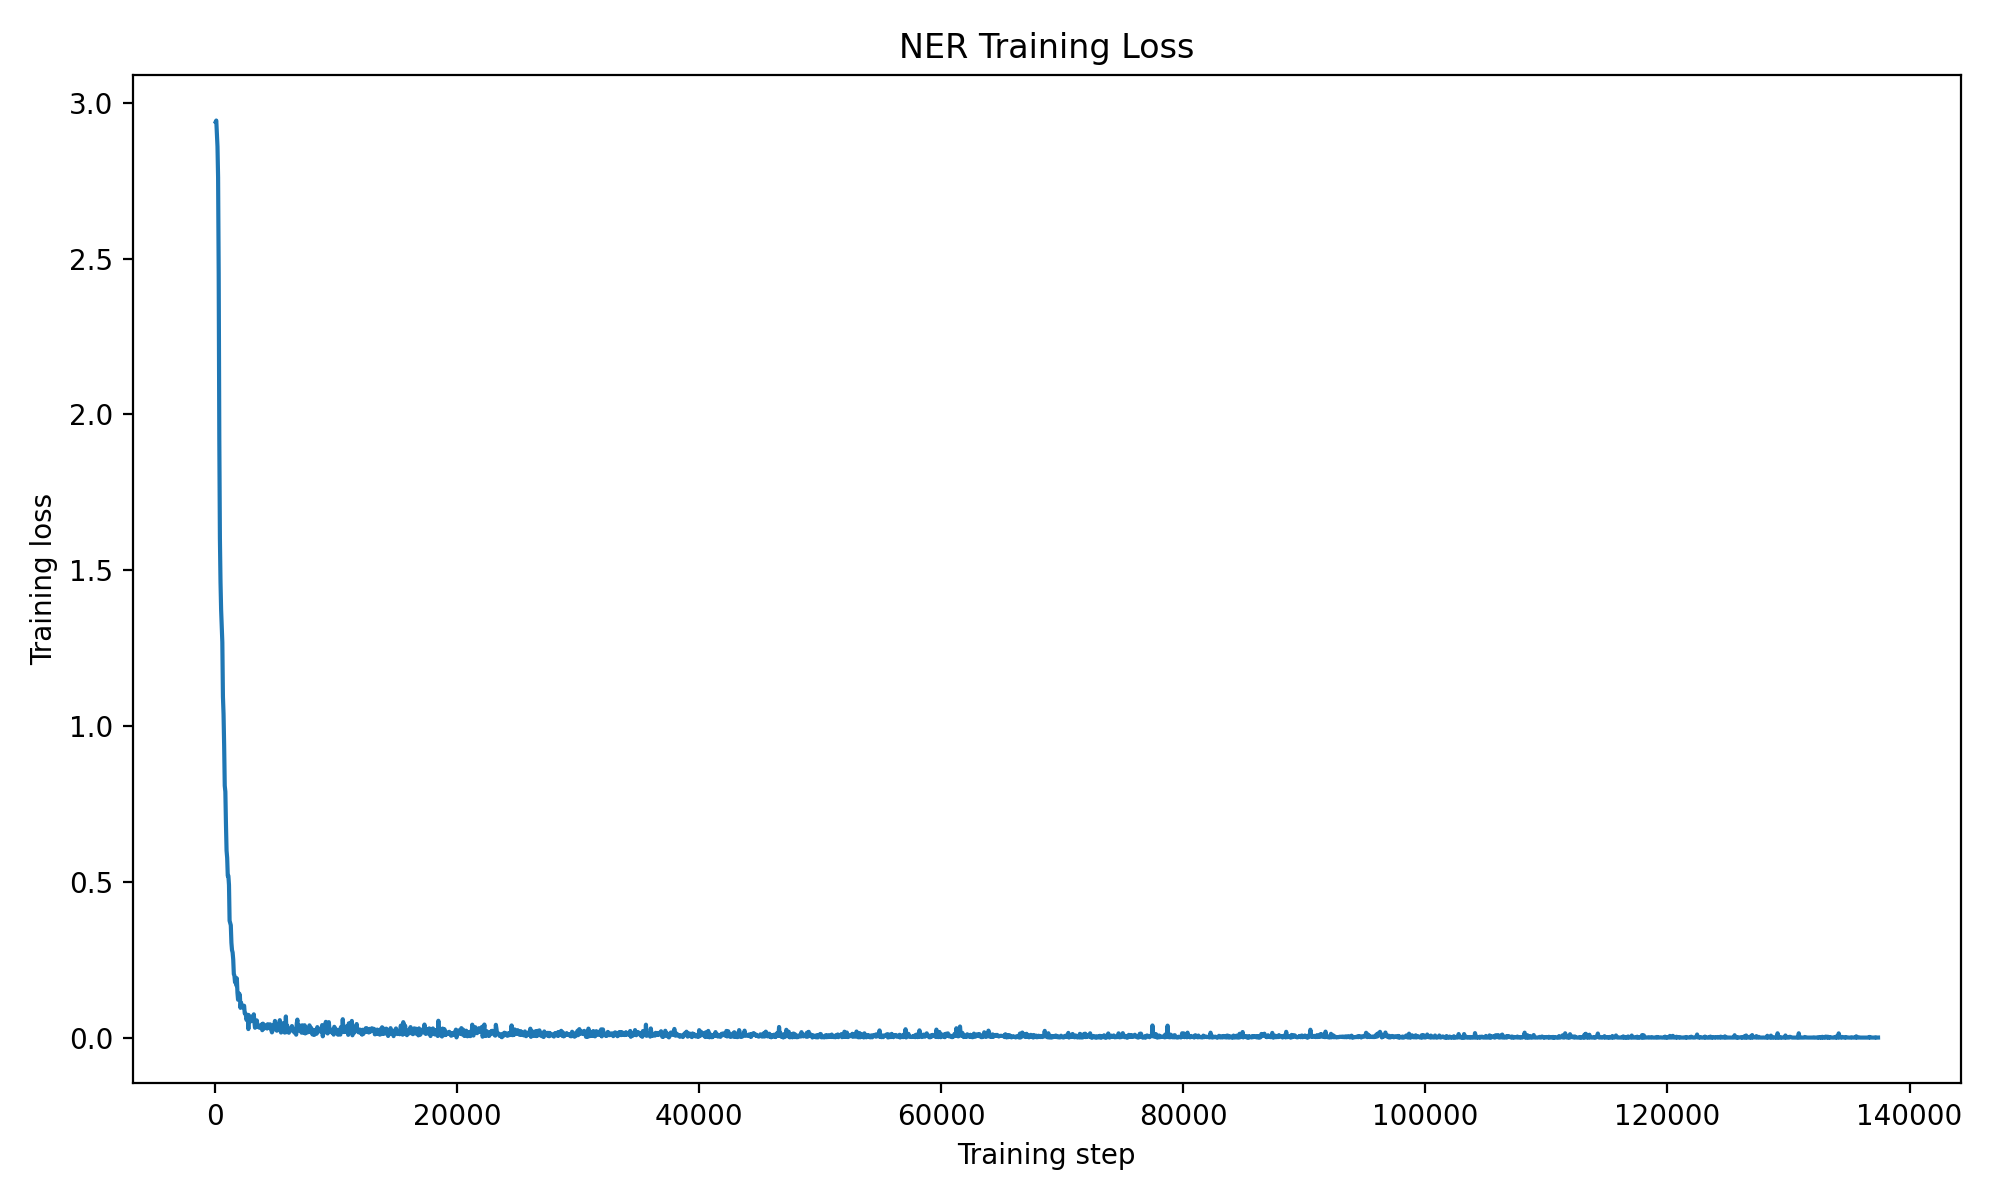
\includegraphics[width=0.82\textwidth]{figures/images/chapter-11/ner/ner_train_loss.png}
\caption{Training loss during fine-tuning of the NER model.}
\label{fig:ner_train_loss}
\end{figure}

\begin{figure}[H]
\centering
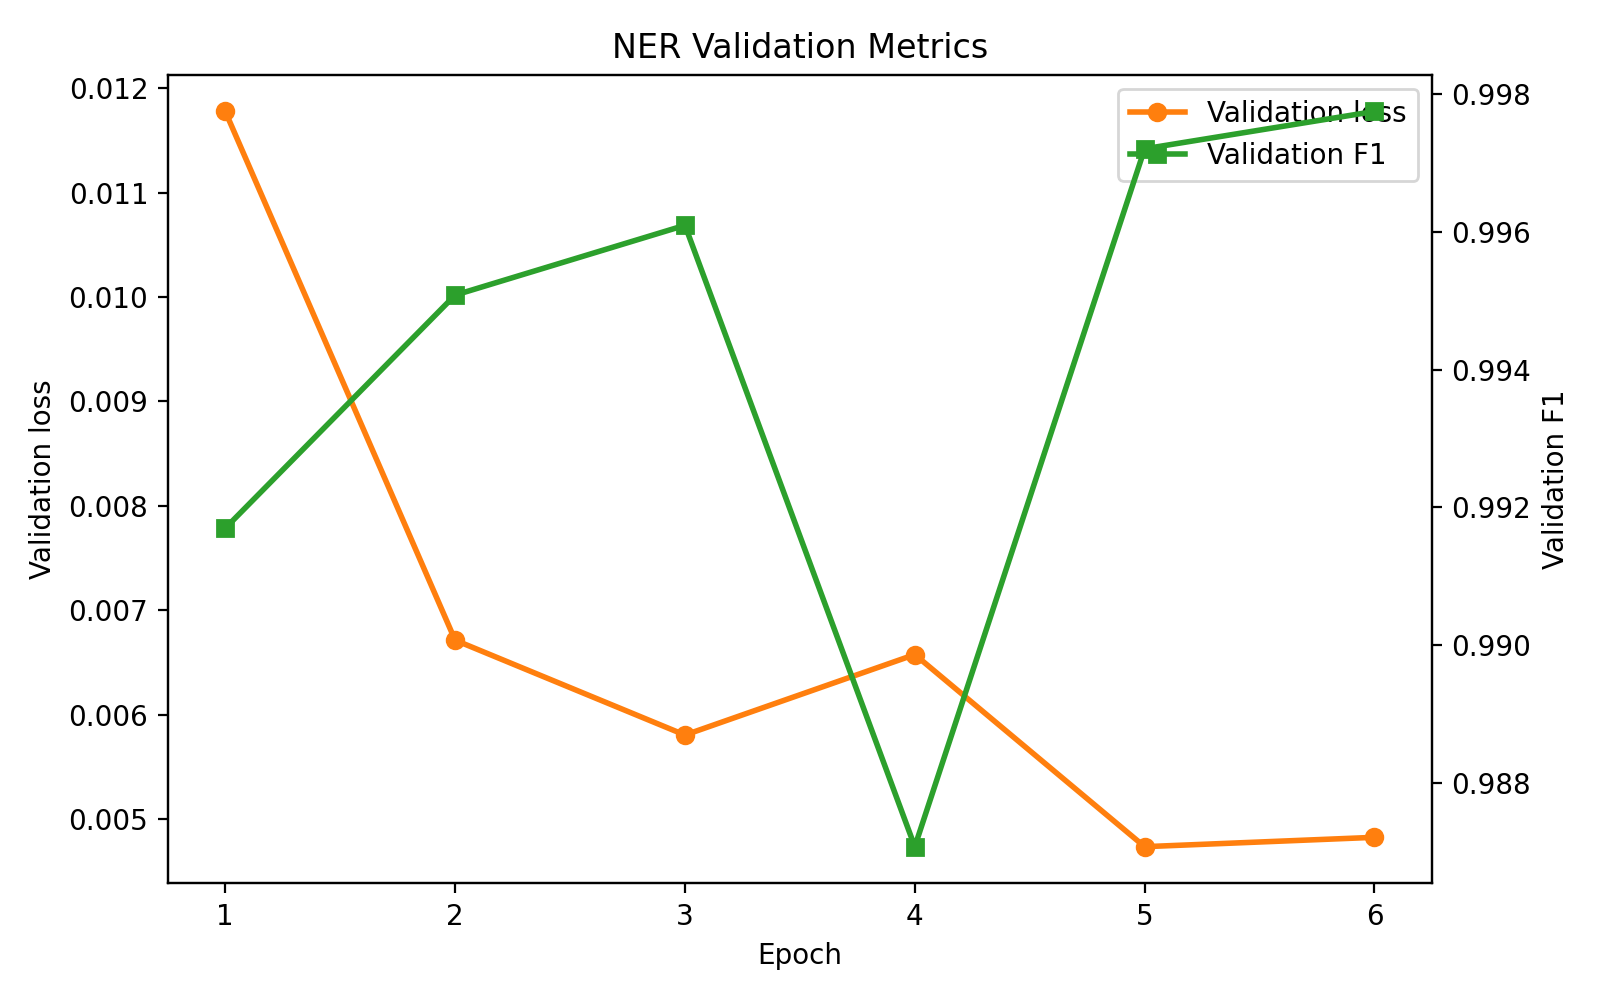
\includegraphics[width=0.78\textwidth]{figures/images/chapter-11/ner/ner_validation_metrics.png}
\caption{Validation loss and validation F1 across training epochs for the NER model. Validation loss is shown on the primary y-axis, while validation F1 is shown on the secondary y-axis.}
\label{fig:ner_validation_metrics}
\end{figure}

Taken together, the curves indicate stable convergence on the constructed training
and validation data, but they do not by themselves demonstrate robust performance
on real-world OCR document scenarios.

\subsection{Per-Label Evaluation}

To better assess generalization, the model was also evaluated on a separate harder
OCR-oriented test set. The overall performance on this set is shown in
Table~\ref{tab:ner_results_hard_appendix}, while the per-label performance is shown
in Table~\ref{tab:ner_hard_test_results} and Figure~\ref{fig:ner_per_label_metrics}.

\begin{table}[H]
\centering
\begin{tabular}{lccc}
\toprule
\textbf{Evaluation set} & \textbf{Precision} & \textbf{Recall} & \textbf{F1 Score} \\
\midrule
Hard test set & 91.32\% & 96.13\% & 0.9366 \\
\bottomrule
\end{tabular}
\caption{Overall NER performance on the harder OCR-oriented test set.}
\label{tab:ner_results_hard_appendix}
\end{table}

\begin{table}[H]
\centering
\begin{tabular}{lcccc}
\toprule
\textbf{Label} & \textbf{Precision} & \textbf{Recall} & \textbf{F1 Score} & \textbf{Support} \\
\midrule
ADDRESS        & 100.00\% & 100.00\% & 1.0000 & 37 \\
DATE           & 100.00\% & 100.00\% & 1.0000 & 50 \\
EMAIL          & 100.00\% & 100.00\% & 1.0000 & 83 \\
ID\_NUMBER     & 90.74\%  & 98.00\%  & 0.9423 & 50 \\
LICENSE\_PLATE & 95.45\%  & 100.00\% & 0.9767 & 21 \\
LOCATION       & 84.21\%  & 88.89\%  & 0.8649 & 72 \\
ORGANIZATION   & 67.16\%  & 95.74\%  & 0.7895 & 47 \\
PERSON\_NAME   & 86.21\%  & 93.75\%  & 0.8982 & 80 \\
PHONE          & 100.00\% & 91.43\%  & 0.9552 & 70 \\
POSTAL\_CODE   & 100.00\% & 100.00\% & 1.0000 & 59 \\
\bottomrule
\end{tabular}
\caption{Per-label performance of the NER model on the harder OCR-oriented test set.}
\label{tab:ner_hard_test_results}
\end{table}

\begin{figure}[H]
\centering
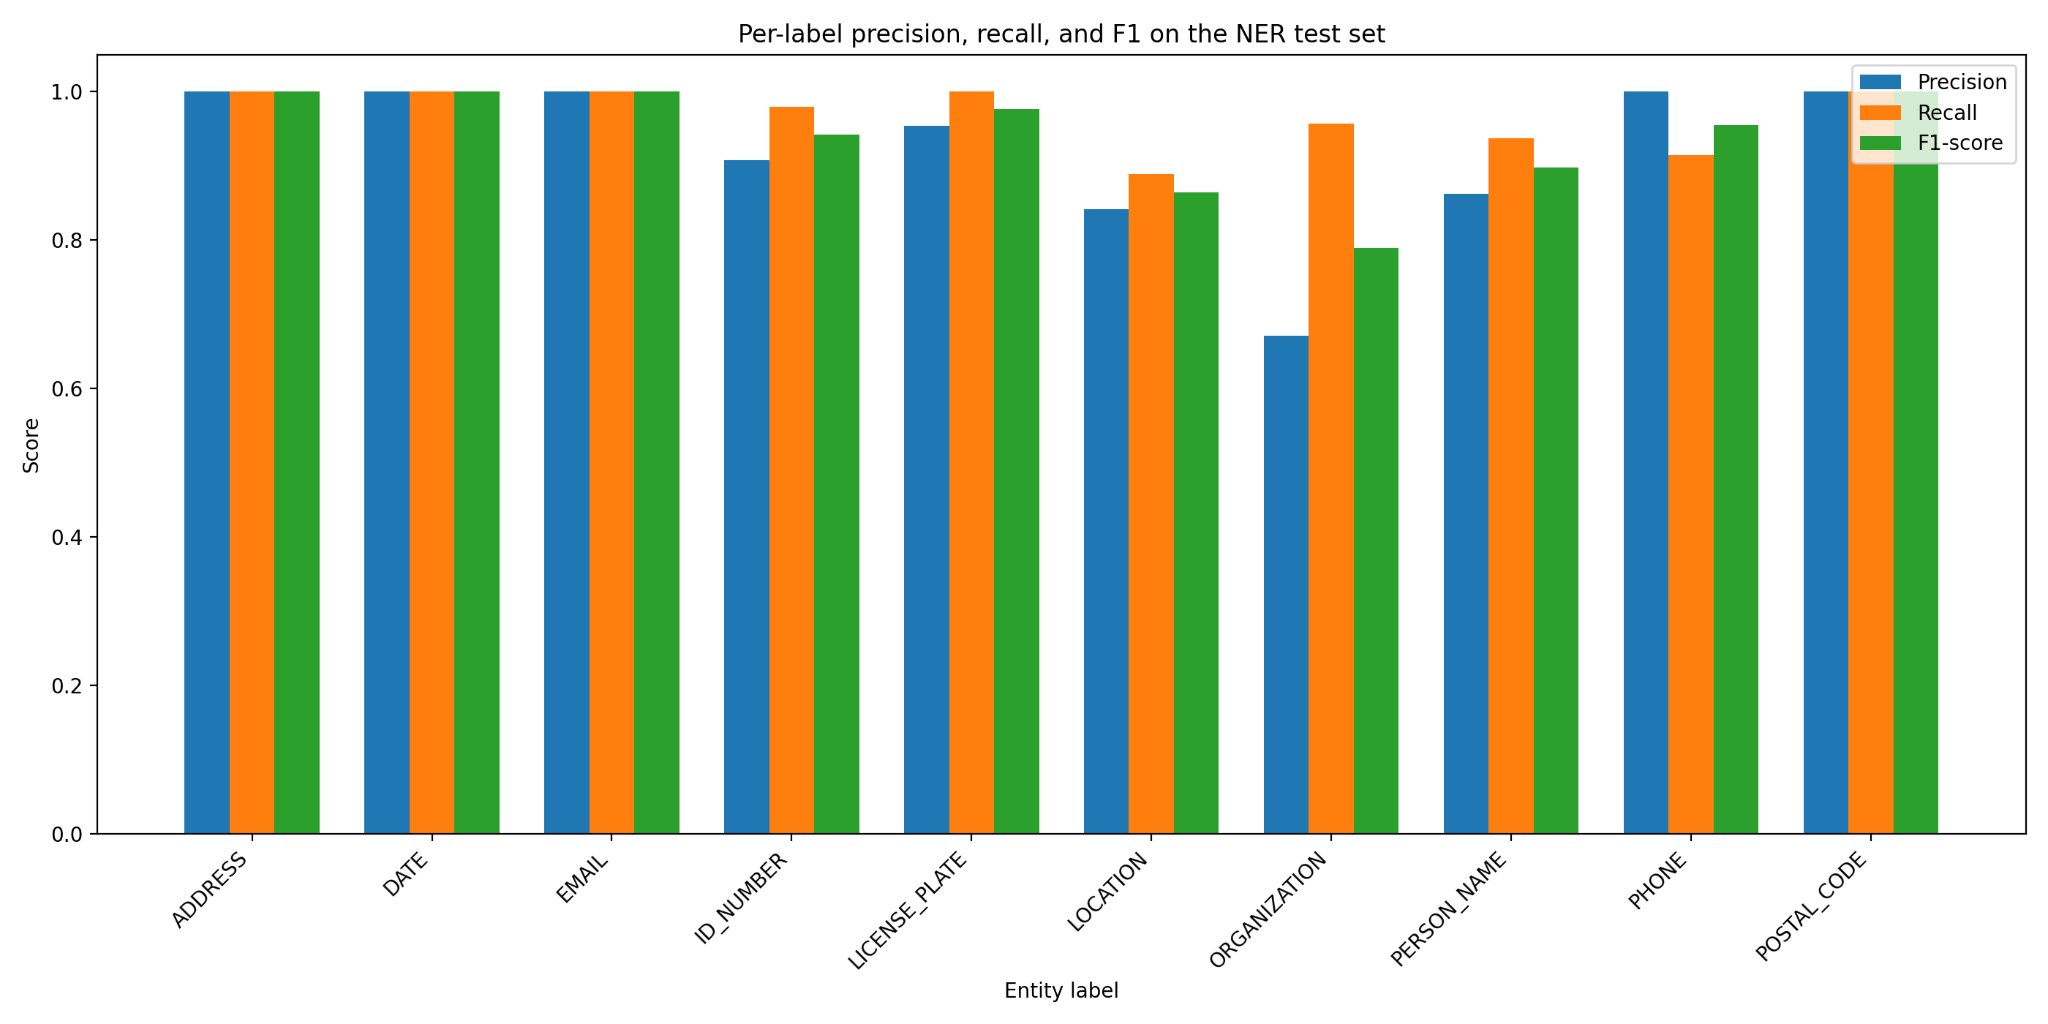
\includegraphics[width=0.9\textwidth]{figures/images/chapter-11/ner/ner_per_label_metrics.png}
\caption{Per-label precision, recall, and F1 on the harder OCR-oriented test set.}
\label{fig:ner_per_label_metrics}
\end{figure}

As shown in Table~\ref{tab:ner_hard_test_results} and
Figure~\ref{fig:ner_per_label_metrics}, the model remained strong on more
structured entity types such as email addresses, postal codes, dates, and
addresses. However, performance was noticeably weaker for semantically more
ambiguous categories such as organizations, locations, and person names. This
indicates that the model generalized less reliably when the OCR text became more
document-oriented and difficult to categorize.

\subsection{Error Analysis}

Figure~\ref{fig:ner_real_vs_controlled } shows a qualitative comparison
between a controlled example and a real-world document scenario. In the
controlled example, the text is more structured and the categorization pipeline
assigns several relevant labels. In the real-world document example, the OCR
text is more fragmented and the assigned categories are less consistent.

These examples illustrate an important limitation of the NER component. While
the model can perform well on structured and simplified inputs, it has greater
difficulty distinguishing reliably between entity categories in practical
document scenarios. This was particularly visible for semantically similar
categories such as person names, organizations, and locations.

\subsection{Summary}

Overall, the NER model achieved very strong results on the constructed held-out
test split and converged stably during training. However, the harder OCR-oriented
evaluation and the qualitative document examples showed that these results
overestimated the practical robustness of the model. In particular, the model
was less reliable for semantically ambiguous categories such as organization,
location, and person-name entities. For this reason, the final SafeVision system
did not rely on the NER model alone, but instead used it as part of a hybrid
text-analysis pipeline.